%% This document gives an example on how to use the ntnubachelorthesis
%% LaTeX document class.
%% Use oneside for PDF delivery and twoside for printing in a book style
%% use language english, norsk, nynorsk and one of the following shortenings
%%  ``BSP'' Bachelor i Spillprogrammering,\\
%%  ``BRD'' Bachelor i drift av nettverk og datasystemer,\\
%%  ``BIS'' Bachelor i Informasjonssikkerhet,\\
%%  ``BPU'' Bachelor i Programvareutvikling, \\
%%  ``BIND'' Bachelor i Ingeniorfad - data, \\
%%  ``BADR'' Bachelor i drift av datasystemer, \\
%%  ``BIT'' Bachelor i informatikk, \\
%%  ``BABED'' Bachelor i IT-støttet bedriftsutvikling.
%%   for example \documentclass[BIS,norsk,twoside]{ntnuthesis/ntnubachelorthesis}

\documentclass[BIS,norsk,oneside]{ntnuthesis/ntnubachelorthesis}
\thesistitle{Case 1: Ulovlig fildeling på universitetsnettet til NTNU}
\thesisshorttitle{Case 1: Ulovlig fildeling på universitetsnettet til NTNU}
\thesisauthor{Thomas Huse, Philip Nyblom, Ole Martin Søgnen, Fredrik Løvaas Theien}
\thesisdate{16.05.2018}

\usepackage{csvsimple}
\usepackage{booktabs}
\usepackage{gnuplottex}
\usepackage[T1]{fontenc}
\usepackage[utf8]{inputenc}     % For utf8 encoded .tex files because...
\usepackage[norsk]{babel}       % For Norwegian labeling
\usepackage{graphicx}           % For inclusion of graphics
\PassOptionsToPackage{hyphens}{url}
\usepackage{url}
\usepackage{hyperref}    % For cross references in pdf
\usepackage{tabularx}
\usepackage[table]{xcolor}
\usepackage{colortbl}
\usepackage{placeins}
\usepackage{pdfpages}
\usepackage{enumitem}
\usepackage{multirow}
\usepackage{lscape}
\usepackage{bigstrut}
\usepackage{verbatim}
\usepackage{float}


\definecolor{darkgreen}{rgb}{0,0.5,0}
\definecolor{apricot}{RGB}{255, 217, 178}

\lstset{        basicstyle=\ttfamily,
                keywordstyle=\color{blue}\ttfamily,
                stringstyle=\color{darkred}\ttfamily,
                commentstyle=\color{darkgreen}\ttfamily,
}


%Typesetting of C++
\newcommand{\CPP}[0]{{C\nolinebreak[4]\hspace{-.1em}\raisebox{.1ex}{\small\bf +\hspace{-.1em}+\ }}}



%\newcommand{\comment}[1]{\textcolor{blue}{\emph{#1}}}  %% use of the colour and you can see how to use commands with parts \comment{so what}

%% The class files defines these two
%% \newcommand{\NTNU}{Norwegian University for Science and Technology} %

% you can create you one #define like structures using the \newcommand feature
% you can change behaviour using \renewcommand

\newcommand{\com}[1]{{\color{red}#1}} % supervisor comment
%\renewcommand{\com}[1]{} %remove starting % to remove supervisor comments
% This will appear in text \com{Lecuters comment} and be visible unless you uncomment
% the renewcommand line.

\newcommand{\todo}[1]{{\color{green}#1}} % items to do
%\renewcommand{\todo}[1]{} %remove starting % to remove items to do

\newcommand{\n}[1]{{\color{blue}#1}} % other comment
%\renewcommand{\n}[1]{} %remove starting % to remove notes

\newcommand{\dn}[1]{} % add the d to a note to say that you have finished with it.

\newcommand{\gj}{NTNU i Gj\o{}vik}


% Norwegian Characters,  needs the {} or to be separate from the next letters
% \o{}   \aa{}   \ae{}   so at the end of a word you can use \o  \aa   \ae
% \O{}   \AA{}   \AE{}   you can also just leave a space and latex will remove it
%    eg, NTNU i Gj\o vik  or NTNU i Gj\o{}vik

\graphicspath{ {bilder/} }

\begin{document}

\thesistitlepage

\tableofcontents
\addtocontents{toc}{\protect\setcounter{tocdepth}{1}}
\listoffigures
\listoftables
%\lstlistoflistings

\chapter*{Kortfattet sammendrag}
Kommer...
\chapter{Introduksjon}
Rotårsaksanalyser er et lite brukt verktøy innen informasjonssikkerhet, men er av økende betydning. Vanlig tilnærming til informasjonssikkerhetsstyring er å utføre en risiko-og sårbarhetsanalyse (ROS-analyse) for så å gjennomføre tiltak som fører risikoene til et akseptabelt nivå. En annen hyppig brukt tilnærming er hendelseshåndtering der en planlegger hvordan det skal responderes på hendelser etter de er inntruffet. Rotårsaksanalyse skiller seg fra disse ved å gå i dybden på problemet, kartlegge hva slags rotårsaker som står bak, og innføre tiltak for å fjerne disse helt.

\section{Oppgavebeskrivelse}
Denne rapporten er en delrapport i en større oppgave om rotårsaksanalyse. Dette caset går inn på rotårsaken til at brukere på skolenettet til NTNU laster ned opphavsrettsbeskyttet materiale. I denne rapporten bruker vi ordet fildeling når vi omtaler deling av filer gjennom torrents. Annen fildeling går ikke under vårt bruk av begrepet og heller ikke under problemstillingen vår. Vi bruker fortsatt begrepet Torrents når vi snakker om selve teknologien og sporingen av dem.

Hver måned får NTNU ca. 150 og 200 unike notifikasjoner om brudd på opphavsretten ved ulovlig fildeling. Vi kan se at dette nummeret går kraftig ned i sommermånedene, som kan tilsi at studentene er hovedgrunnen til bruddene på opphavsrett. Se figur \ref{fig:copyright} under for en grafisk illustrasjon av antall notifikasjoner for brudd på opphavsrett.

\begin{figure}[H]
    \centering
    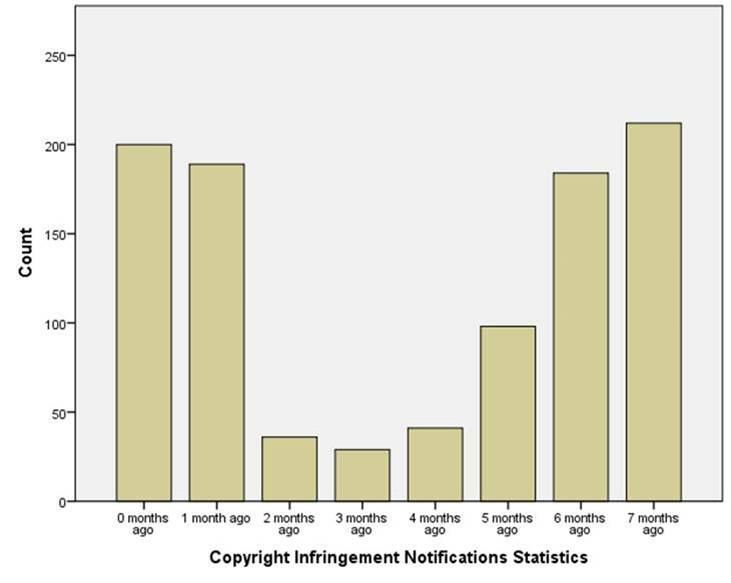
\includegraphics[scale=0.8]{copyright}
    \label{fig:copyright}
    \caption[Copyright Infringement Notifications]{Copyright Infringement Notifications}
\end{figure}

\begin{comment}
\begin{table} [h]
    \begin{tabular}{ | m{12em} | m{12em} | m{12em} | }
        \hline
            \cellcolor{yellow} & \cellcolor{yellow} Breaches & \cellcolor{yellow} Copyright breach/Piracy\\
        \hline
            Policy Violation & Information Security Policy & 2 \\
        \hline
             & IT Policy & 43 \\
        \hline
    \end{tabular}
    \caption{Oversikt over kvantiteten av brudd på policy}
    \label{kritisk_tabell_1}
\end{table}
\end{comment}

I denne oppgaven er vårt mål å finne rotårsakene til ulovlig fildeling og ikke å avdekke noen for det. Derfor er alle spørreundersøkelser anonyme. Dette presiseres også til intervjuobjektene under intervjuet.

\section{Metode}
Metodebruken i denne undersøkelsen er delt inn i syv steg som vist i figur \ref{fig:prosess} under. I hvert steg av denne prosessen brukes det ulike verktøy for å hjelpe til med å forstå problemet, finne rotårsak, og tilslutt implementere tiltak for å eliminere årsakene. 
\begin{figure}[H]
    \centering
    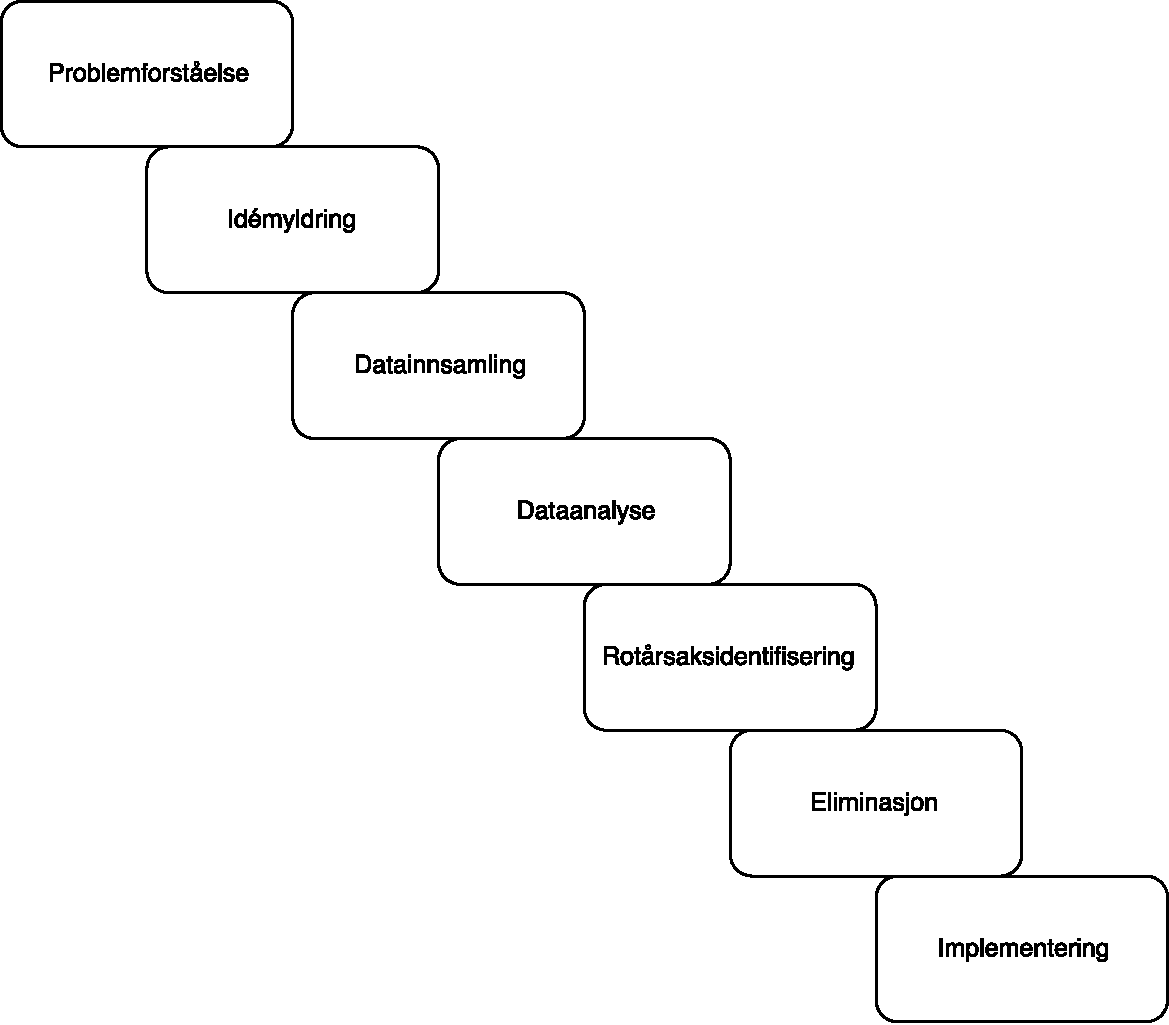
\includegraphics[scale=0.6]{prosess}
    \label{fig:prosess}
    \caption[Rotårsaksanalyseprosessen]{Rotårsaksanalyseprosessen definert av Andersen og Fagerli}
\end{figure}
\chapter{Problemforståelse}

\chapter{Idémyldring}
I dette steget i prosessen er målet å generere en liste over det vi tror kan være mulige årsaker til problemet. Det er en del forskjellige verktøy en kan bruke for å oppnå dette, men vi har valgt å benytte Idémyldring på bakgrunn av verktøyets egenskap til å generere mange idéer hurtig.

\section{Idémyldring}
I rotårsaksanalyse finnes det to ulike måter å gjennomføre Idémyldring på, Strukturert- og Ustrukturert Idémyldring. I den strukturerte versjonen får hver deltaker sin tur til å komme med en idé, og dette sikrer at alle får delta like mye. På den ustrukturerte måten kan alle komme med idéer når de dukker opp, og fungerer mye mer spontant enn den strukturelle. Det er spesielt viktig å ikke omformulere eller diskutere forslagene etterhvert som de kommer, dette skal gjøres etter Idémyldringsøkten er over.

\subsection{Ønsket utbytte}
Ønsket utbytte i denne delen er en mengde idéer som kan legges til grunn når det utføres statistisk arbeid på rotårsakene. Det er spesielt ønskelig å kunne ende opp å utvikle spørsmål til brukerundersøkelser basert på noen av disse årsakene.

\subsection{Gjennomførelse}
Det første som ble gjort når økten startet var å kommunisere og skrive opp problemstillingen på en tavle. Vi valgte å strukturere Idémyldringen som et tankekart ettersom dette var en kjent løsning for gruppen, og brukte den ustrukturerte tilnærmingen til Idémyldringen på grunn av dens uformelle og spontane natur. 

Det første problemet vi så på var hvorfor personer bruker Torrents til å laste ned opphavsrettsbeskyttet materiale. Når idéstrømmen begynte å gå langsomt, stoppet vi og vurderte det vi hadde kommet fram til. Vi kom blant annet fram til at vi burde spesifisere problemstillingen ytterligere og valgte derfor å spesifisere den til hvorfor folk laster ned på skolenettet. Vi forkortet dette til: ``Hvorfor Torrenting på skolenettet'' for enkelthets skyld. Det ble kjørt enda en økt med denne nye problemstillingen og fikk mer spesifikke resultater. 

\subsection{Resultater}
Etter øktene var ferdig ble det gjort en vurdering av resultatene og de ble kategorisert i henhold til likhetstrekk, under en fellesnevner som for eksempel Økonomi. Resultater og gruppering er som vist i figur \ref{fig:idemyldring} under.

\begin{figure}[H]
    \centering    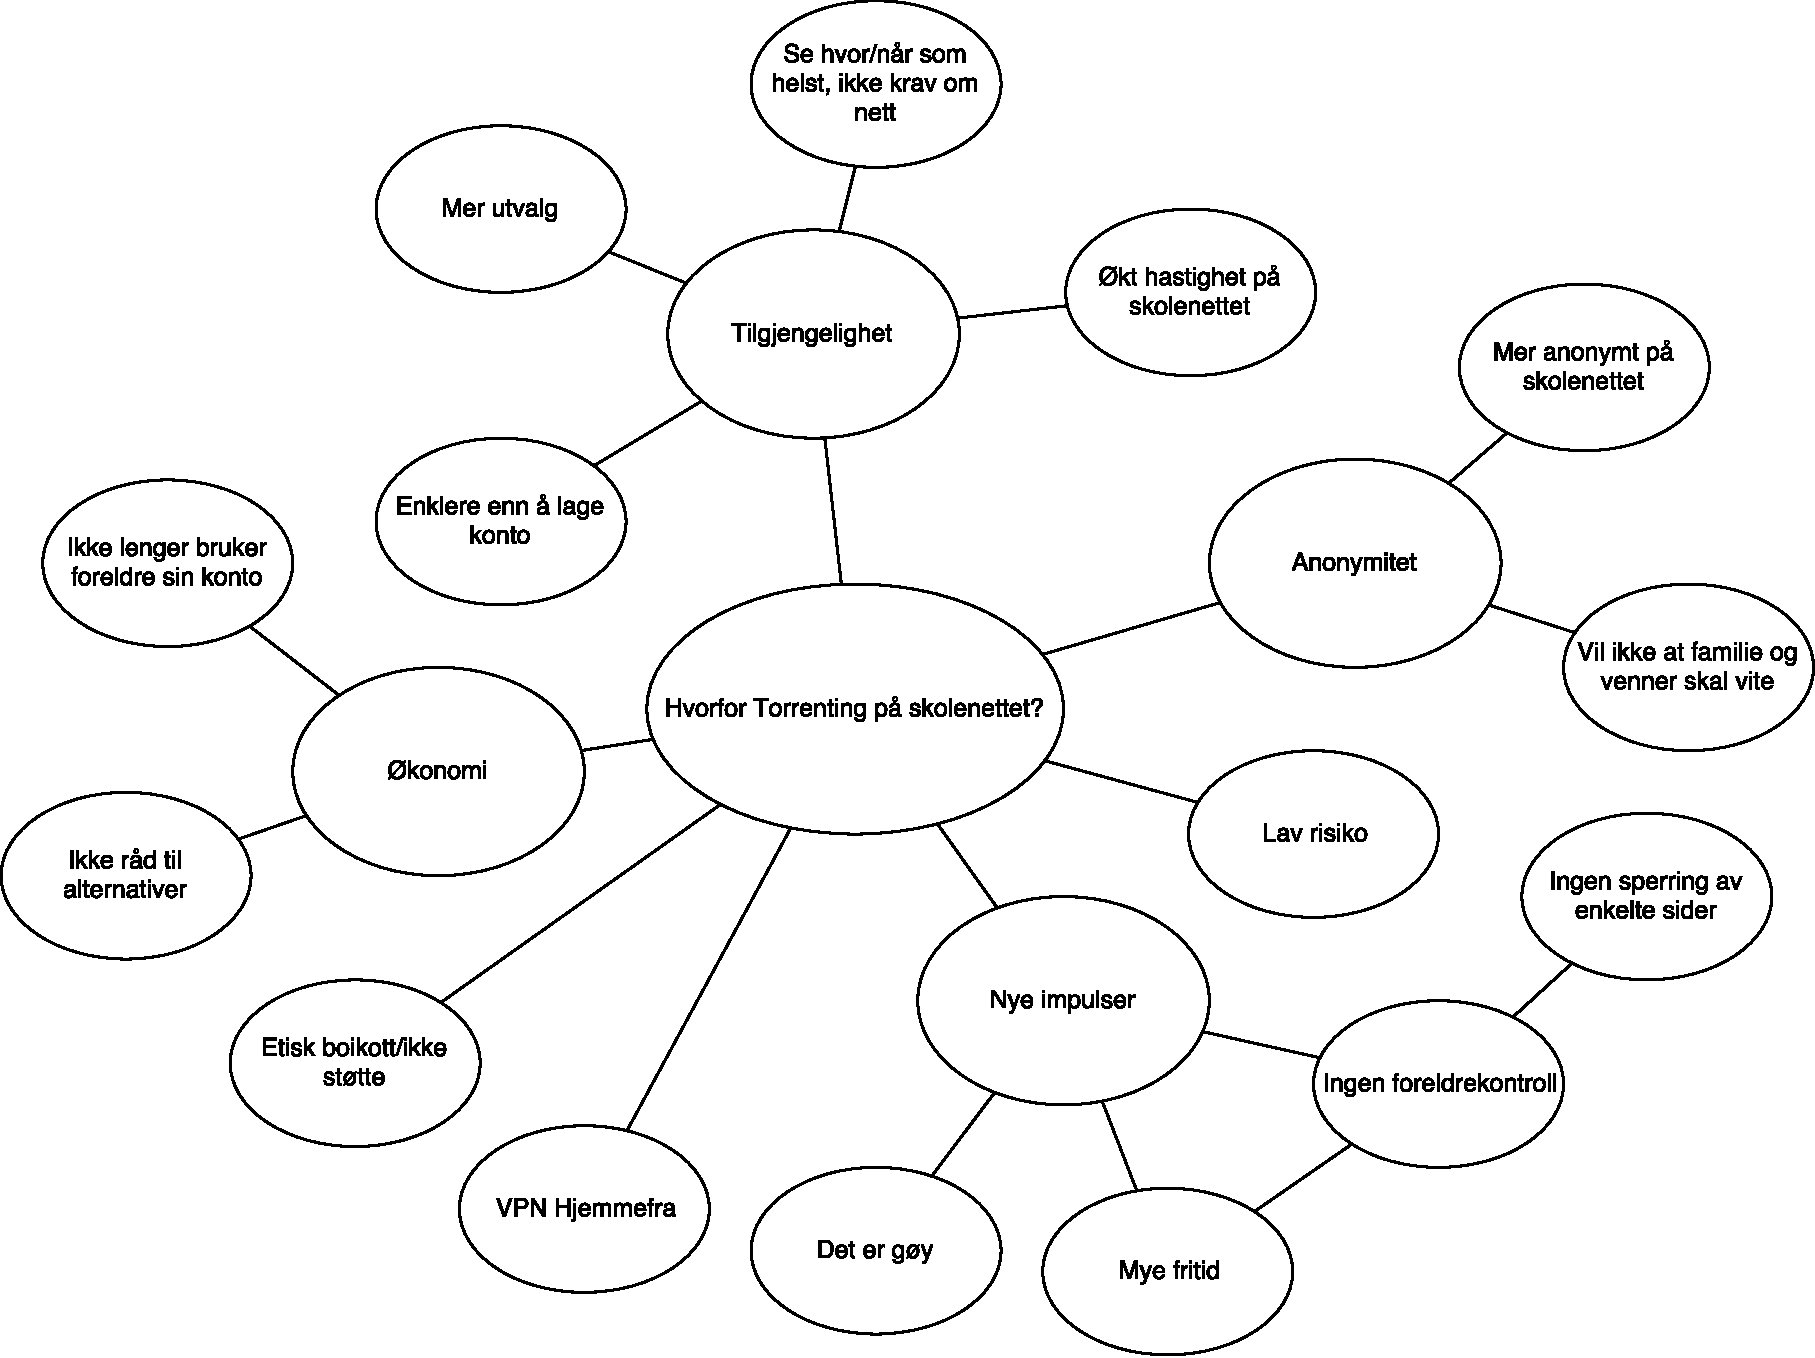
\includegraphics[scale=0.45]{case_1/bilder/idemyldring}
    \caption[Idémyldring]{Resultater og gruppering av idémyldringen}
    \label{fig:idemyldring}
\end{figure}

Resultatene er gruppert inn i fire hovedkategorier, Økonomi (som går på kjøpekraften til den enkelte person), Tilgjengelighet (hvor god tilgang en har på tjenester), Anonymitet (foreldre kunne blant annet overvåke før, samt føler seg tryggere når det er flere på samme nett) og Nye impulser (mer frihet og fritid, og påvirkning av nedlastningskulturen).

Merk at noen årsaker kunne ikke plasseres i én kategori og er derfor direkte knyttet til problemstillingen. 


\subsection{Konklusjon av verktøyet}
Dette var en effektiv metode for å få en overordnet oversikt av hva årsakene kan være til at noen velger å laste ned opphavsrettsbeskyttet materiale, spesielt på skolenettet. Verktøyet fungerte bra i denne sammenhengen fordi gruppen hadde en del basiskunnskap om temaet fra før. Vi antar at en slik metode vil fungere dårligere dersom problemet ikke er forstått godt nok og/eller det er lite kunnskap om problemstillingen på forhånd.
\chapter{Datainnsamling}
Datainnsamlingen er kritisk til resultatet av oppgaven. Målet i denne fasen er å samle inn et så bredt aspekt av informasjon som mulig gjennom et par mulige verktøy og teknikker beskrevet i boka om rotårsaksanalyse\cite{RCA}. Vi har valgt å bruke spørreundersøkelser som et verktøy for å hente inn informasjon om dette caset fordi vi skal hente inn informasjon fra et stort antall studenter som bor i studentbyene SiT administrerer.

\section{Elektronisk spørreundersøkelse}
Det finnes i hovedsak to forskjellige undersøkelsestyper, kvantitative og kvalitative spørreundersøkelser. Kvalitative undersøkelser går ut på å spørre utvalgte personer, og er ofte mye mer detaljerte og samler svar av høyere kvalitet. Kvantitative undersøkelser fungerer motsatt i at det er fokus på mange tilbakemeldinger slik at en kan senke usikkerhet knyttet til svarkvalitet. \cite{} I vår situasjon har vi valgt kvantitativ undersøkelse på bakgrunn av et par faktorer. For det første ønsker vi at undersøkelsen skal være helt anonym, siden spørsmålene omhandler potensielle lovbrudd. For det andre er målgruppen et stort antall personer, så det kan være nyttig å samle inn data fra så mange av de som mulig.

\subsection{Ønsket utbytte}
Det vi ønsker å få ut av spørreundersøkelsen er data på utvalgte spørsmål vi mener er relevante for oppgaven. Denne fasen er utelukkende for å innhente informasjon, bearbeiding av informasjonen skjer i neste fase. Spørsmålene er utarbeidet for å utforske hvorfor studenter som bor i studentbyer laster ned opphavsrettsbeskyttet materiale, som blant annet inkluderer undersøkelse av økonomiske perspektiver og tilgjengelighet på tjenester. I tillegg ønsker vi også innsikt i hvordan dette kan stoppes. 

Hypotesen vi går inn i undersøkelsen med er at folk laster ned opphavsrettsbeskyttet materiale fordi det er lett tilgjengelig, tilknyttet liten til ingen kostnad og ikke minst fordi det er svært lav risiko for represalier.

\subsection{Gjennomførelse}
Prosessen startet ved å utforme spørreundersøkelsen. En god undersøkelse vil alltid kreve kartlegging av demografi, og i vår undersøkelse valgte vi å kartlegge studentby, kjønn, alder og fakultet. Kjønn og alder er ganske selvforklarende, mens studentby ble valgt på bakgrunn av at Kallerud har mye raskere nedlasting- og opplastingshastighet enn de andre stedene. Vi anså også at det ville være forskjell på hvor mange som laster ned mellom for eksempel informatikkstudiene og helsestudiene. Videre ble resultatene i de foregående fasene brukt til å utforme spørsmålene. Spørreundersøkelsen inkluderer spørsmål om hvor godt en rekke påstander stemmer for den enkelte der respondentene svarer på en likert-skala fra 1-5, der 1 er i liten grad og 5 er i stor grad. Til slutt inkluderes det et spesielt viktig spørsmål om hva som skal til for at personen stopper med ulovlig nedlasting. Dette er et frisvar der vi kommer til å analysere individuelle svar hver for seg. Spørreundersøkelsen kan leses i sin helhet i \hyperref[undersokelse]{Vedlegg A}.
\newline
Det er alltid en stor utfordring å finne nok respondenter til spørreundersøkelser, og vi setter en del krav til antall respondenter og utfører en rekke tiltak for å oppnå nok besvarelser, slik at undersøkelsen kan si noe om rotårsaken med relativt høy sikkerhet. Det er et krav å få minst 30 besvarelser som hadde lastet ned opphavsrettsbeskyttet materiale mens de har bodd i hybelen. Videre er det også ønskelig med relativ likhet i antall respondenter mellom de ulike fakultetene og studentbyene. Det hadde vært ideelt med minst 30 respondenter i hver kategori her også, men det er ønsketenkning i denne sammenhengen. Under prosessen ble også totalt antall beboere fra alle studentbyene i SiT bolig kartlagt. Boligtorget ga oss innbyggertallene fra hver studentby, og vi regnet oss frem til totalt 522 beboere. Det er viktig å presisere at det kan være usikkerheter knyttet til disse tallene, siden det kan hende ikke alle boligene har en beboer.

Siden spørreundersøkelsen er elektronisk var et av de første tiltakene som ble gjennomført å spre den på relevante facebook-sider. Et av prosjektgruppens medlemmer jobber på Studenthuset her på Gjøvik, og fikk spørreundersøkelsen delt på deres facebook-side. Senere i prosessen ble også undersøkelsen delt på facebook-siden til linjeforeningen INGa og klassesidene til sykepleierne og webutvikling. Undersøkelsen ble også delt gjennom venner og bekjente; disse var for det meste informatikkstudenter. I tillegg ble det laget en plakat som ble hengt opp på oppslagstavler på skolen og i vaskeriene i de ulike studentbyene, og mange ble også plassert i postkassene til SiT boliger. Plakaten finnes i \hyperref[plakat]{Vedlegg B}. 

\subsection{Resultater}
Undersøkelsen endte med 97 svar totalt, dette er 18.6\% av de 522 beboerne i SiT bolig. Av disse var det 34 som svarte at de hadde lastet ned opphavsrettsbeskyttet materiale i hybelen, det er 35\% av de spurte. Videre resultater og analyse av disse blir diskutert i neste fase. 

\subsection{Konklusjon av verktøy}
Konklusjonen er at spørreundersøkelser er en effektiv metode for å samle inn store mengder data. En må likevel være konsekvent på tiltakene som iverksettes for å få inn respondenter. Det er også viktig i kvantitative spørreundersøkelser å få relativ likhet i demografien for å kunne si noe om de ulike kategoriene. Dette kan i noen tilfeller være krevende. En annen ting som er svært sentralt i bruk av verktøyet er utformingen av spørsmålene. Det er vanskelig å legge til spørsmål etter spørreundersøkelsen allerede er utsendt, og hva en da trenger ekstra informasjon må dette supplementeres i en mulig kvalitativ undersøkelse eller liknende. 
\chapter{Dataanalyse}
I denne fasen analyseres vi dataene som er samlet inn, vi har ganske lite data i dette caset, derfor har vi ganske få valgmuligheter for bruk av verktøy i følge boken \cite{RCA}. Dataene er heller ikke på nummerisk form, som flere av analyseverktøyene krever.

\section{Affinitetsdiagram}
Affinitetsdiagram brukes til å analysere data som det ikke er mulig å nummerere, eksempelvis meninger eller ideer. Affinitetsdiagram grupperer data og finner de underliggende korrelasjoner og likhetstrekk i gruppen.


\section{Ønsket utbytte}
Ønsket utbytte av å bruke affinitetsdiagram er å finne bindinger eller fellesnevnere som kan være til hjelp for å fjerne rotårsaken. 

\section{Gjennomføring}
Analysen ble gjennomført med å ta transkripsjon av intervjuet og stykke den opp i fem hovedgrupper.     

\section{Resultat}

\begin{figure}[H]
    \centering
    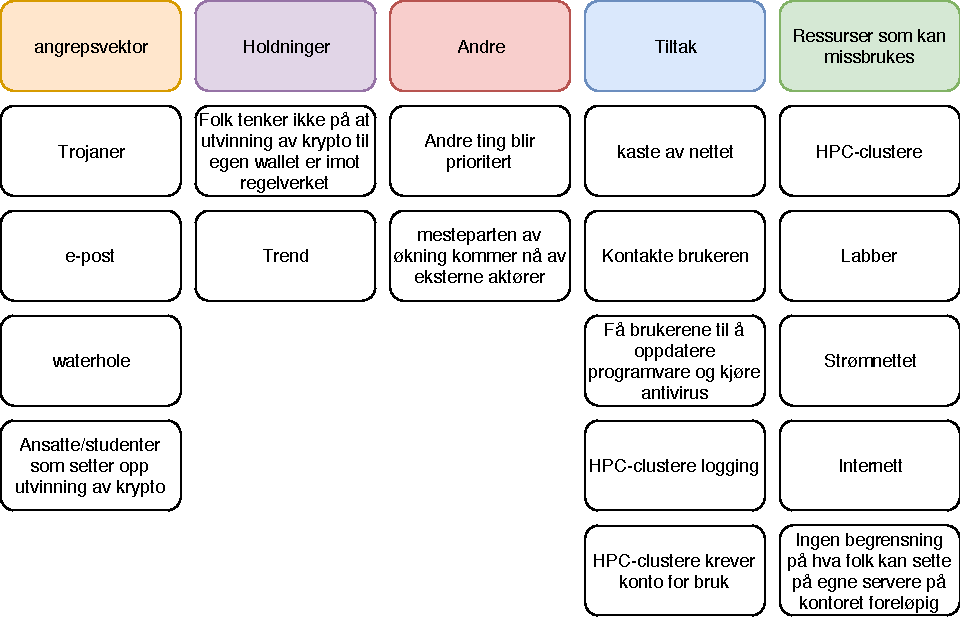
\includegraphics[scale=0.6]{case_3/bilder/AD.pdf}
    \label{fig:AD_miner}
    \caption[Analyse av intervju]{Hvordan fungerer utvinning av kryptovaluta ved NTNU?}
\end{figure}

Vi finner mulige årsaker og tiltak som er satt på plass, og forhåpentligvis er rotårsaken blant dem.

\section{Konklusjon av verktøy}
Verktøyet fungerte godt, selv med en liten datamengde. Vektøyet er effektivt til å strukturere transkripsjonen fra intervjuet til mer brukbare og oversiktlige nøkkelpunkter. 

\chapter{Rotårsaksidentifisering}
Arbeidet i denne fasen går ut på å identifisere rotårsaken. I foregående fasen ble en rekke mulige årsaker identifisert og analysert, men nå er det tid for å finne den faktiske rotårsaken. Det er mange forskjellige verktøy som kan brukes i denne fasen, men vi har brukt et årsak-virkningsdiagram for vårt utgangspunkt.

\section{Årsak-virkningsdiagram}
Et årsak-virkning diagram er et diagram som analyserer forholdene mellom et problem og dets årsaker. Det kombinerer aspekter ved idémyldring med systematisk analyse. Det finnes to typer årsak-virkning diagrammer, fiskebeindiagram og prosessdiagram. Mens et prosessdiagram er mer direkte fokusert på problemet på innsiden av forretningsprosessene, er et fiskebeindiagram en mer generell tilnærming for å adressere alle potensielle årsaker\cite{RCA}. I dette caset har vi valgt et fiskebeindiagram på bakgrunn av at årsakene er spredt over flere variabler. 

\subsection{Ønsket utbytte}
Ved bruk av dette verktøyet ønsker vi å sitte igjen med en visuell fremstilling av rotårsakene til problemet. Dette vil gjøres ved å identifisere hva som skaper årsakene vi har funnet fram til i foregående fase. 

\subsection{Gjennomføring}
Det er anbefalt å bruke en tusjtavle for å tegne opp fiskebeindiagrammet, men vi valgte å bruke det nettbaserte programmet draw.io \cite{drawio}. Draw.io er laget for å skape diagrammer med flere brukere involvert i sanntid. De hadde en egen mal for fiskebeindiagram som vi valgte å gå ut fra. Stegene vi fulgte i prosessen er hentet fra boka om rotårsaksanalyse \cite{RCA} og ble som følger:

\begin{enumerate}
    \item Først ble problemet definert og skrevet i slutten av fiskebeindiagrammet.
    \item Deretter ble hovedkategoriene skrevet ned i bokser. Disse er direkte tilknyttet resultatene fra analysen.
    \item Videre startet vi å idémyldre alle mulige årsaker under hver kategori, en kategori om gangen. Disse ble fortløpende skrevet inn i diagrammet.
    \item Til slutt analyserte vi de identifiserte årsakene og bestemte de mest sannsynlige rotårsakene
\end{enumerate}

\subsection{Resultat}
Innledningsvis ble problemet beskrevet som rotårsaken til kompromitterte kontoer ved NTNU. Hovedkategoriene som ble undersøkt for å finne svar på dette, var gjenbruk av innloggingskredentialier tilhørende NTNU, IT-reglementet og andre styringsdokumenter, passordvaner, phishing og oversikt. Både hovedkategoriene og årsakene under disse er i hovedsak basert på dataanalysen, mens noe er basert på kreativ idémyldring. 

\begin{figure}[H]
    \centering
    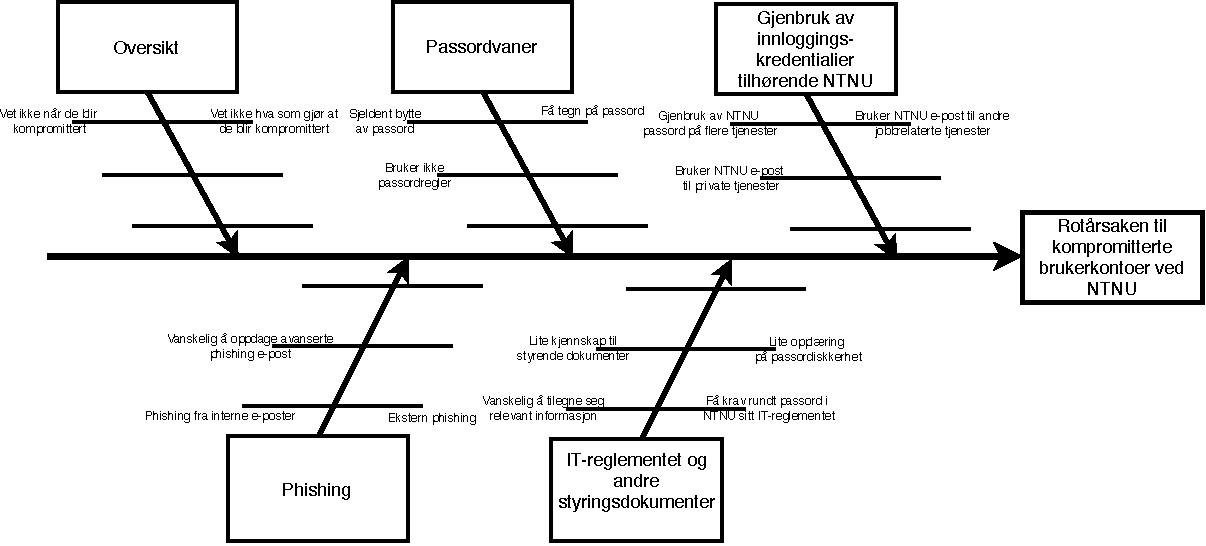
\includegraphics[scale=1.1, angle=90]{case_2/bilder/fiskebein.pdf}
    \label{fig:fiskebein-case2}
    \caption[Fiskebein-case2]{Fiskebeindiagram over hovedkategorier og årsaker}
\end{figure}

Vi har kommet frem til at rotårsaken til kompromitterte kontoer er sammensatt av flere faktorer. Et passord på mellom åtte til elleve tegn i seg selv er ikke nok for at kontoen skal bli kompromittert, men sammen med at de bytter sjeldnere enn hvert andre år gjør at dette blir et problem. I tillegg til dette bruker flertallet NTNU e-posten til andre tjenester, enten til jobbrelatert eller til privat bruk. De bruker også samme NTNU passord på flere tjenester. Dette er noe en burde unngå til en hver tid, og er noe av det vi anser å være blant det mest kritiske. 

Respondentene hadde også liten kjennskap til IT-reglementet og andre styringsdokumenter. De svarte også at de har fått lite opplæring på passordsikkerhet. Vi har lest igjennom IT-reglementet og andre styringsdokumenter, og har kommet frem til at IT-reglementet har for få krav til passord, det var vanskelig å tilegne seg all informasjon på de forskjellige styringsdokumentene da IT-reglementet ikke henviste til noen av retningslinjene. I Retningslinjer for behandling av brukernavn, passord og andre autentiseringsdata \cite{RetnBPA} står det at passordet skal byttes hver 12 måned. Denne retningslinjen er ikke nevnt i IT-reglementet at du skal gjøre deg bekjent med. 

Sammenlagt så viste det oss at respondentene hadde dårlige passordvaner, gjenbruk av innloggingskredentialier tilhørende NTNU og lite kunnskap til IT-reglementet og andre styrende dokumenter. Phishing er også en relevant årsak til kompromitterte kontoer. Phishing e-poster har blitt såpass sofistikerte at det er vanskelig å skille mellom falske og legimite e-poster. \cite{SophPhish}. Rotårsakene er derfor som følger: 

\begin{itemize}
    \item Mistet kontodetaljer av phishing
    \item E-post og passordgjenbruk på andre tjenester
    \item Liten kjennskap til IT-reglement og andre styrende dokumenter
    \item Dårlige passordvaner
\end{itemize}

\subsection{Konklusjon av verktøy}
Verktøyet fungerte veldig bra, siden det var så mange faktorer som kunne være rotårsakene. Det var litt vanskelig å gruppere hovedkategoriene i dette caset, fordi mange av årsakene kunne plasseres i flere hovedkategorier. Dette skyldes at problemet er spredt over flere årsaker som påvirkes av hverandre. Etter hovedkategoriene var definert var det enkelt å belyse årsaker, på grunn av gode data i dataanalysen. 

\section{5 Whys}
5 Whys er et verktøy som prøver å gjøre et dypdykk i årsakene for å finne rotårsaken. Måten dette gjøres på er å hele tiden spørre ``Why?'', altså hvorfor på norsk, hver gang en ny årsak dukker opp. Det brukes ofte for å sjekke om de identifiserte årsakene er symptomer, lav-nivå årsaker eller rotårsaker. 

\subsection{Ønsket utbytte}
Ved å bruke 5 Whys er det ønskelig å konfirmere om årsakene som ble fremhevet i fiskebeindiagrammet er faktiske rotårsaker, eller bare symptomer og/eller lav-nivå årsaker. 

\subsection{Gjennomføring}
Med dette verktøyet tar vi utgangspunkt i casebeskrivelsen, nemlig rotårsaken til kompromitterte kontoer ved NTNU. Ut fra dette brukte vi årsaker fra fiskebeindiagrammet over for å komme på årsaker som skal analyseres, samt prøvde å idémyldre et par nye. For hver av disse årsakene ble det spurt: ``Hvorfor er dette en årsak av det orginale problemet?''. For hvert svar spør vi hvorfor igjen og igjen helt til vi finner rotårsaken. Det ble tatt utgangspunkt i fem iterasjoner, men det er mulighet for fler eller færre avhengig av om spørsmålet kan besvares på en fornuftig måte. 

\subsection{Resultater}
Det ble fremhevet fem årsaker som skulle analyseres. Fire av disse kom fra fiskebeindiagrammet over, og en fra idémyldring. Tabellene under viser resultatene fra gjennomføringen. 

\begin{table} [H]
    \centering
    \begin{tabular}{ | m{5em} | m{30em} | }
        \hline
            \cellcolor{yellow} Årsak: & \cellcolor{yellow} Mistet kontodetaljer av phishing                \\
        \hline
            Why? & Fordi e-posten kom fra en intern e-postadresse                                   \\
        \hline
            Why? & Fordi kontoen var blitt kompomittert                                             \\
        \hline
            Why? & Fordi kontodetaljene ble phishet fra en ekstern e-postadresse                \\
        \hline
            Why? & Fordi brukeren var ikke oppmerksom på at det var en phishing e-post              \\
        \hline
            Why? & Fordi brukeren hadde ikke fått tilstrekkelig opplæring i deteksjon av phishing e-post    \\
        \hline
    \end{tabular}
    \caption[5 Whys: Mistet kontodetaljer av phishing]{5 Whys på mistet kontodetaljer av phishing}
    \label{5Whys-phishing}
\end{table}

Å miste kontodetaljer av en phishing e-post kan skje fra enten interne eller eksterne e-postadresser. I 5 Whys over kom vi frem til at dette skjer fordi en ikke er oppmerksom på tvilsomme e-poster. Årsaken til det kan være fordi brukerne ikke har fått tilstrekkelig opplæring i deteksjon av phishing e-post.

\begin{table} [H]
    \centering
    \begin{tabular}{ | m{5em} | m{30em} | }
        \hline
            \cellcolor{yellow} Årsak: & \cellcolor{yellow} E-post og passordgjenbruk på andre tjenester \\
        \hline
            Why? & Fordi det er vanskelig å huske mange unike brukerdetaljer \\
        \hline
            Why? & Fordi det ikke brukes passordmanager \\
        \hline
            Why? & Fordi de ikke vet hva det er \\
        \hline
            Why? & Fordi det ikke gis informasjon om det i retningslinjene \\
        \hline
            Why? & - \\
        \hline
    \end{tabular}
    \caption[5 Whys: E-post og passordgjenbruk på andre tjenester]{5 Whys på e-post og passordgjenbruk på andre tjenester}
    \label{5Whys-phishing}
\end{table}

Årsaken til at mange velger å benytte samme kredentialer flere steder er som regel at de synes det er vanskelig å huske mange brukerdetaljer, og motsatt, enkelt å huske få. Noe som kan gjøre dette lettere er å bruke en passordmanager, men dette informeres det ikke om i styringsdokumentene. 

\begin{table} [H]
    \centering
    \begin{tabular}{ | m{5em} | m{30em} | }
        \hline
            \cellcolor{yellow} Årsak: & \cellcolor{yellow} Liten kjennskap til IT-reglement og andre styrende dokumenter \\
        \hline
            Why? & Fordi det er vanskelig å tilegne seg informasjon \\
        \hline
            Why? & Fordi informasjonen er spredt på mange sider og dokumenter \\
        \hline
            Why? & Fordi det ikke er et overordnet ISMS \\
        \hline
            Why? & - \\
        \hline
            Why? & - \\
        \hline
    \end{tabular}
    \caption[5 Whys: Liten kjennskap til IT-reglement og andre styrende dokumenter]{5 Whys på liten kjennskap til IT-reglement og andre styrende dokumenter}
    \label{5Whys-phishing}
\end{table}

En mulig årsak til at det er liten kjennskap til disse dokumentene er at det er vanskelig å tilegne seg informasjonen. Det blir ofte mye for en person å forholde seg til, spesielt når informasjonen er spredt utover mange forskjellige sider og dokumenter. Et overordnet ISMS kunne hjulpet med å standardisere sikkerhetsstyringen, og kanskje sentralisere informasjonen. 

\begin{table} [H]
    \centering
    \begin{tabular}{ | m{5em} | m{30em} | }
        \hline
            \cellcolor{yellow} Årsak: & \cellcolor{yellow} Dårlige passordvaner \\
        \hline
            Why? & Fordi de er lite bevisste på sikkerhet \\
        \hline
            Why? & Fordi de tenker det ikke er så viktig \\
        \hline
            Why? & Fordi det er ingen tydelige krav rundt passord i NTNU sitt IT-reglement \\
        \hline
            Why? & Fordi IT-reglementet ikke henviser til de relevante dokumentene \\
        \hline
            Why? & - \\
        \hline
    \end{tabular}
    \caption[5 Whys: Dårlige passordvaner]{5 Whys på dårlige passordvaner}
    \label{5Whys-passordvaner}
\end{table}

Mange har dårlige passordvaner, fordi de er lite bevisste på sikkerhet, og at de ikke tenker det er så viktig. Mulig årsak til dette kan være fordi det ikke er noen tydelige krav rundt passord i NTNU sitt IT-reglement. IT-reglementet henviser ikke til de dokumentene som nevner passordrutiner \cite{ITReg}, og det er bare IT-reglementet brukerne er pliktig å sette seg inn i og skrive under på \cite{}. 

\begin{table} [H]
    \centering
    \begin{tabular}{ | m{5em} | m{30em} | }
        \hline
            \cellcolor{yellow} Årsak: & \cellcolor{yellow} Lukrativt for trusselaktører \\
        \hline
            Why? & Fordi de tjener og sparer penger på å kompromittere kontoer \\
        \hline
            Why? & Fordi de får tilgang til forskningsdatabaser \\
        \hline
            Why? & Fordi det er for enkelt å få tilgang til brukerkontoene \\
        \hline
            Why? & Fordi det er utilstrekkelig tilgangskontroll på brukerkontoene \\
        \hline
            Why? & - \\
        \hline
    \end{tabular}
    \caption[5 Whys: Lukrativt for datakriminelle]{5 Whys på lukrativitet for datakriminelle}
    \label{5Whys-passordvaner}
\end{table}

Det er lukrativt for datakriminelle å prøve å kompromittere brukerkontoer fordi det er for god kost-nytte effekt. De kan tjene penger på å selge kontoene, eller spare penger ved å laste ned forskningsartikler. Her kom vi frem til at utilstrekkelig tilgangskontroll kan være en rotårsak til at det er så høy kost-nytteverdi for trusselaktørene.

\subsection{Konklusjon av verktøy}
Verktøyet var svært nyttig for å gå dypt inn i årsakene. Et problem består ofte av flere nivåer av årsaker, og det tar 5 Whys hensyn til. I forhold til informasjonssikkerhet burde man passe på å ikke alltid ende opp med en årsak som er relatert til Policy, da problemet ofte også kan være av teknisk art. Det var en mulig fallgruve for oss, men det er usikkert om det bare gjelder dette caset. Et annet problem med verktøyet er at det kan bli for enssporet på en spesifikk tankegang. Det kan derfor anbefales i noen tilfeller å undersøke samme årsaken flere ganger dersom det er grunn til å tro at det finnes flere relevante årsaker ved ett av spørsmålene, som fører til en annen rotårsak. 

\chapter{Rotårsakseliminering}
Denne fasen går ut på å finne tiltak som kan eliminere rotårsakene til kompromitterte kontoer ved NTNU. 

\section{Systematisk Innovativ Tenkning (SIT)}
Systematic Inventive Thinking inneholder fem hovedprinsipper:

\begin{enumerate}
    \item \textbf{Attributtavhengighet} Endre på en essensiell variabel.
    \item \textbf{Komponentkontroll} Ser på hvordan et produkt er tilknyttet omgivelsene sine.
    \item \textbf{Erstatning} Bytte ut en del av produktet med noe i omgivelsene til produktet.
    \item \textbf{Forkastning} Fjerne en del av produktet for å bedre det.
    \item \textbf{Oppdeling} Prøver å splitte et produkts attributter i to.
\end{enumerate}

\subsection{Ønsket utbytte}
Ved å bruke SIT metoden ønsker vi å få kreative idéer på hvordan vi kan finne en løsning til kompromitterte kontoer ved NTNU. 

\subsection{Gjennomføring}
SIT burde helst gjennomføres av 10-12 personer, fra en rekke forskjellige fagområder, men siden vi ikke hadde så mange tok vi bare utgangspunkt i prosjektgruppen. 
\subsubsection{Komponenter} 
Her blir alle komponenter som omhandler problemet listet.

\begin{itemize}
    \item E-postadresse
    \item Brukernavn
    \item Autentisering
    \item IT-reglement
    \item Retningslinjer for behandling av brukernavn, passord og andre autentiseringsdata
    \item Prinsipper for informasjonssikkerhet (inkludert Policy)
    \item Påloggingssystem
    \item E-post filter
\end{itemize}

Når komponentene er gjort rede for, vil de fem SIT prinsippene brukes sekvensielt på komponentene for å utvikle løsninger på problemene. Resultatene fremheves i neste seksjon. 


\subsection{Resultater}
Ikke alle SIT-prinsipper finner løsninger som er gjennomførbare for alle komponenter. I disse tilfellene vil det stå: ``Ikke gjennomførbart''. 

\paragraph{E-post}
\begin{itemize}
    \item \textbf{Attributtavhengighet} Ikke gjennomførbart.
    \item \textbf{Komponentkontroll} Bevisstgjøringskampanje for god e-postskikk.
    \item \textbf{Erstatning} Gi folk kurs og hjelp til å ordne private e-postadresser.
    \item \textbf{Forkastning} Ikke gjennomførbart.
    \item \textbf{Oppdeling} Gi folk en egen epost adresse som bare skal brukes til privat bruk.
\end{itemize}

\paragraph{Brukernavn}
\begin{itemize}
    \item \textbf{Attributtavhengighet} Ikke gjennomførbart.
    \item \textbf{Komponentkontroll} Ikke gjennomførbart.
    \item \textbf{Erstatning} Ha mer tilfeldig brukernavn som er vanskeligere å gjette.
    \item \textbf{Forkastning} Ikke la e-postadressen kunne brukes som brukernavn.
    \item \textbf{Oppdeling} Ikke gjennomførbart.
\end{itemize}

\paragraph{Autentisering}
\begin{itemize}
    \item \textbf{Attributtavhengighet} Krav om sterkere passord.
    \item \textbf{Komponentkontroll} Bruke passordmanager for å behandle passord. 
    \item \textbf{Erstatning} Ikke gjennomførbart.
    \item \textbf{Forkastning} Ikke gjennomførbart.
    \item \textbf{Oppdeling} Gå over til 2-faktor autentisering.
\end{itemize}

\paragraph{IT-reglement}
\begin{itemize}
    \item \textbf{Attributtavhengighet} Utbedre IT-reglementet med tydeligere krav rundt passord. 
    \item \textbf{Komponentkontroll} Henvise til de andre styringsdokumentene.
    \item \textbf{Erstatning} Ikke gjennomførbart.
    \item \textbf{Forkastning} Ikke gjennomførbart.
    \item \textbf{Oppdeling} Ikke gjennomførbart.
\end{itemize}

\paragraph{Retningslinjer for behandling av brukernavn, passord og andre autentiseringsdata}
\begin{itemize}
    \item \textbf{Attributtavhengighet} Ikke gjennomførbart.
    \item \textbf{Komponentkontroll} Bevisstgjøringskampanje.
    \item \textbf{Erstatning} Legge retningslinjene inn i IT-reglementet.
    \item \textbf{Forkastning} Ikke gjennomførbart.
    \item \textbf{Oppdeling} Ikke gjennomførbart.
\end{itemize}

\paragraph{Prinsipper for informasjonssikkerhet}
\begin{itemize}
    \item \textbf{Attributtavhengighet} Ikke gjennomførbart.
    \item \textbf{Komponentkontroll} Integrere det i et ISMS
    \item \textbf{Erstatning} Ikke gjennomførbart.
    \item \textbf{Forkastning} Ikke gjennomførbart.
    \item \textbf{Oppdeling} Ikke gjennomførbart.
\end{itemize}

\paragraph{Påloggingssystem}
\begin{itemize}
    \item \textbf{Attributtavhengighet} Øk minimum antall tegn på passord fra 8 til 10. 
    \item \textbf{Komponentkontroll} Overholde kravet om å bytte passord hver 12. måned.
    \item \textbf{Erstatning} Ikke gjennomførbart. 
    \item \textbf{Forkastning} Ikke gjennomførbart. 
    \item \textbf{Oppdeling} Enhetskontroll på nye innlogginger.
\end{itemize}

\paragraph{E-post filter}
\begin{itemize}
    \item \textbf{Attributtavhengighet} Forbedre e-post filter.
    \item \textbf{Komponentkontroll} Ikke gjennomførbart. 
    \item \textbf{Erstatning} Ikke gjennomførbart. 
    \item \textbf{Forkastning} Ikke gjennomførbart. 
    \item \textbf{Oppdeling} Ikke gjennomførbart. 
\end{itemize}

Vi sorterer og beskriver de mest relevante idéer til videre utdyping:

\begin{description}
\item[Bevisstgjøringskampanje for god e-postskikk]
Med god e-postskikk så mener vi at brukerene er bevisste på om e-post er legitim eller ikke, og at NTNU e-post ikke skal bli benyttet til andre tjenester.

\item[Gi folk kurs og hjelp til å ordne private e-postadresser]
Det er et problem at folk bruker sin NTNU e-post til andre tjenester. Dette kan være fordi de ikke har en egen privat e-post de kan bruke til dette. Dette tiltaket vil hjelpe de med å anskaffe en privat e-post, så de ikke bruker NTNU e-posten på andre ting en det den er ment for.

\item[Ikke la e-postadressen kunne brukes som brukernavn]
Dersom e-postadressen er brukt på andre tjenester med samme passord som NTNU, kan trusselaktørene også kompromittere NTNU kontoen. Hvis ikke e-postadressen lar seg bruke som brukernavn, vil det senke risikoen for at de får logget seg på. 

\item[Krav om sterkere passord]
Krav om sterkere passord i form av økt minimumslengde fra 8 til 10 tegn. 

\item[Overholde kravet om å bytte passord hver 12. måned]
I retningslinjene for behandling av autentiseringsdata er det krav om å bytte passord hver 12. måned. Dette blir ikke håndhevet. Et mulig tiltak er derfor å automatisk kreve endring av passord hver 12. måned. 

\item[Gå over til 2-faktor autentisering]
For å hindre at kontoen blir kompromittert dersom passordet ble det kan man benytte seg av 2-faktor autentisering. Dette skaper ekstra redundans. 

\item[Bruke passordmanager for å behandle passord]
Det blir lettere å behandle lange, kompliserte og unike passord med en passordmanager. 

\item[Utbedre IT-reglementet med tydeligere krav rundt passord]
Per nå er det eneste som står i IT-reglementet rundt passord at man skal bytte passord dersom man har mistanke om at noen vet det. Dette mener vi ikke er nok, og burde utbedres, for eksempel ved å referere til retningslinjer for behandling av autentiseringsdata. 

\item[Henvise til de andre styringsdokumentene]
Per nå er det lite henvisning til andre styringsdokumenter som gjør det vanskelig og tungvint for brukerene å lete igjennom dokumentene. Dette burde samles på ett sted og henvise til hverandre.

\item[Bevisstgjøringskampanje rundt autentiseringsdata]
Bevisstgjøringskampanjen skal få frem at passordet til NTNU kontoen skal ikke bli brukt til andre tjenester for å sikre at uvedkommende ikke får tilgang til kontoen.

\item[Integrere Prinsipper for informasjonssikkerhet i et ISMS]
Etter hva vi har fått av informasjon fra oppdragsgiver har ikke NTNU et skikkelig ISMS. Dette er noe som før eller siden bør være på plass. 

\item[Enhetskontroll på nye innlogginger]
En mulig måte å gjennomføre dette på er å sende en e-post eller sms om å autorisere enheten når det er første gang du logger på, på den enheten. Eventuelt validere den for 30 dager av gangen før dette må gjøres på nytt. 

\end{description}

\subsection{Tiltaksplan}
Etter å ha brukt de fem SIT-prinsippene på hver komponent, og filtrert de, sitter vi igjen med et par idéer. I denne delen fremhever vi idéer i en tiltaksplan som vi anbefaler å implementere. 
Under beskrives de ulike tiltakene:

\begin{description}
    \item[Bevisstgjøringskampanje for god e-postskikk og behandling av autentiseringsdata] Denne bevisstgjøringskampanjen vil inkludere opplæring i deteksjon av phishing e-post, beste praksis innen behandling av brukernavn, passord og andre autentiseringsdata, og innsikt i eksisterende dokumentasjon som NTNU har på informasjonssikkerhet. 
    \item[Krav om strengere passordkontroll] Dette tiltaket vil inkludere en økning av minimum passordlengde fra 8 til 10 tegn, og innføre en automatisk funksjon som pålegger deg å bytte passord hver 12. måned, slik det er krav om i retningslinjene. 
    \item[Implementer 2-faktor autentisering] Tiltaket går ut på å implementere 2-faktor autentisering for hver innlogging. Vi anbefaler å bruke sms, som gir deg en kode du kan logge inn med. 
    \item[Enhetskontroll og informering på nye innlogginger] Dette tiltaket går på å ha en enhetskontroll der ansvarlig bruker får sms når noen logger inn fra en ny enhet. Dersom dette var et legitimt påloggingsforsøk fra brukeren kan han/hun validere enheten for en gitt periode. Vi anbefaler 30 dager av gangen, men dette kan muligens også spesifiseres av brukeren. 
    \item[Utbedre IT-reglement til å inkludere og samle retningslinjer og krav] Dette tiltaket går på å utbedre passordkrav i tillegg til å henvise retningslinjer og andre styrende dokumenter. Dette burde samles på èn Innsida-side slik at det er lett å finne frem de nødvendige dokumentene til informasjonssikkerhet. 
    \item[Anbefale brukere å benytte passordmanager] Dette tiltaket går på å inkludere passordmanager som et anbefalt verktøy på samlesiden til IT-reglementet, retningslinjer og andre styrende dokumenter
\end{description}

\subsection{Konklusjon av verktøy}
På mange av komponentene var det vanskelig å finne tiltak og løsninger til hver av de fem hovedprinsippene. Dette førte til at det ble ganske mange steder vi måtte skrive ``Ikke gjennomførbart''. Enkelte av prinsippene kunne også være mer relevant for en spesifikk komponent som gjorde at det kunne være flere tiltak på ett prinsipp. Ellers fant vi mange gode tiltak som vil enten fjerne rotårsakene eller senke risikoen til at dette skjer. 
\chapter{Løsningsimplementering}
Arbeidet i denne fasen går ut på å utrede en tiltaksplan og lage et forslag til hvordan dette skal implementeres. I den foregående fasen ble løsningene til rotårsaken identifisert til å være at alt materiale blir gratis og tilgjengelig på ett sted, tilby produkter fra selskap som universitetet får flest notiser fra, kurs for studenter i bruk av universitetsnettet og bytte av ISP på Sit-boligene. Kurs for studenter og bytting av ISP vil kunne stoppe NTNU fra å motta notifikasjoner for brudd på opphavsrett, men vil ikke nødvendigvis stoppe beboere fra å laste ned. 

\section{Tiltaksplan}
Gjennomføring av disse tiltakene vil i hovedsak administreres av universitetet og Sit.

\subsection{Alt av materiale blir gratis og tilgjengelig på ett sted}
Dette tiltaket vil fjerne rotårsaken helt og holdent. Alt materiale blir gratis, gitt ut på samme tid over hele verden og tilgjengelig på ett sted. Dette tiltaket har svært høy kost, men også høy nytte. Skolen må skaffe avtaler med alle produsenter og tilby det til studentene. 

\subsection{Tilby produkter fra selskap som universitetet får flest notiser fra}
Finne ut de mest populære selskapene som universitetet får notis fra, og skaffe en avtale med rettighetshaverne eller som er distributør for rettighetshaverene og gjøre dette tilgjengelig for studenter. Dette vil fjerne rotårsaken på at de laster ned fra dette selskapet. Dette har lav start kostnad som starter med å kartlegge hvilke firmaer som har høy frekvens av notiser. Kostnaden tilknyttet dette tiltaket er i hovedsak det å få til en avtale med rettighetshaverene, eller distributørene av materialet i Norge.

\subsection{Kurs for studenter i bruk av universitetsnettet}
Etablere et kurs for studenter om hvordan man skal bruke universitetsnettet. Nye studenter som kommer til NTNU vil ha som krav å gjennomføre kurset, som en del av signereingen av IT reglementet. Kurset vil avluttes med en test, for å se hvor mye av IT reglementet studenten har fått med seg. Denne testen kan muligens brukes i forbindelse med inititav/straff ettersom hvor godt studenten gjør det. Dette kurset kan bli for omfattende for hele universitetet og kan heller bare bli gitt til Sit leietakere. Dette prosjektet kan bli både tidkrevende og ha en høy kostnad, så vi foreslår for å begrense ressursbruken at dette prosjektet blir en mulig bacheloroppgave.   

\subsection{Sit bytter ISP}
Det å bytte ISP eller splitte studenthjemmene fra skolenettverket vil være en dyr og tidkrevende prosess, men dette kan være verdt å gjennomføre. Dette vil ikke fjerne rotårsaken til problemet, men vil flytte problemet vekk fra NTNU.


\section{Trediagram}
Trediagram benyttes for å lage en liste over aktiviteter som må gjennomføres for å implementere tiltaket. Trediagram er en ekstremt enkel prosjektplan.

\subsection{Ønsket utbytte}
Ønsket utbytte ved å bruke trediagram er å få en liste over aktiviteter som må bli gjennomført for å innføre det spesifikke tiltaket.   

\subsection{Gjennomføring}
Dette verktøyet startet med å gruppere hovedtiltak til rotårsaken, deretter ble hver aktivitet som må gjennomføres for at tiltaket skal bli gjennomført gruppert. Disse underpunktene ble gruppert etter hvilken rekkefølge de skal bli implementert slik at tiltaket er mulig å gjennomføre. 

\subsection{Resultater}
Dette ga oss en fullstendig plan over hvilke aktiviteter som må gjennomføres for at tiltaket skal bli implementert. 

\begin{figure}[H] 
    \centering    
    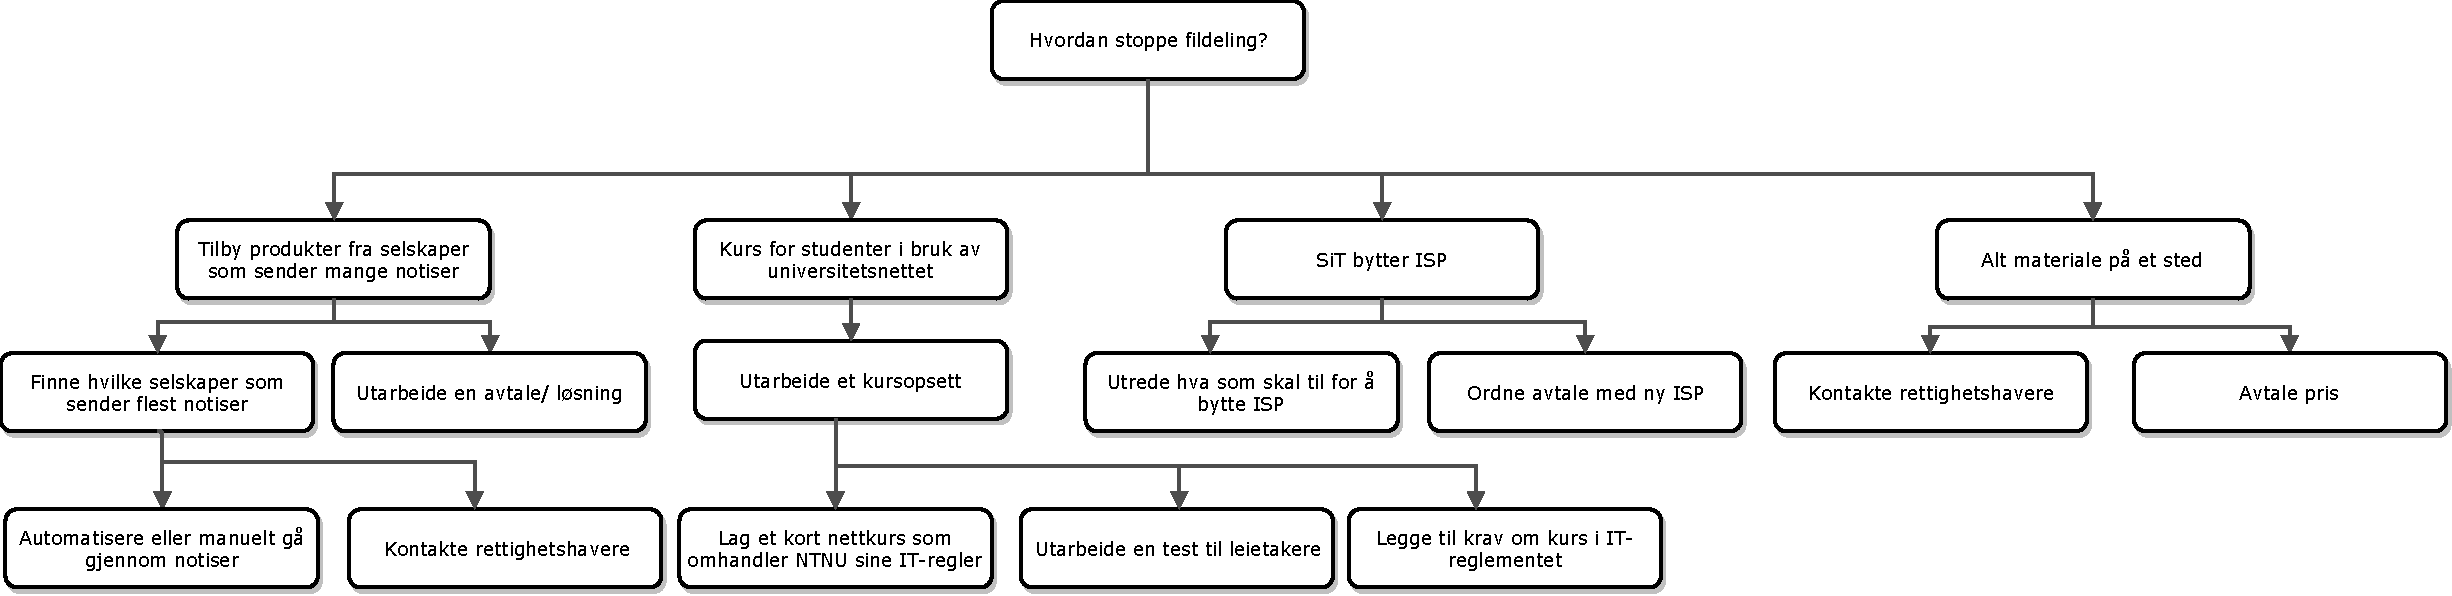
\includegraphics[scale=0.55, angle=90]{case_1/bilder/Tre-diagram.pdf}
    \caption[Trediagram til tiltak for case 1]{Løsningsimplementering}
    \label{fig:Tre-diagram}
\end{figure}

\subsection{Konklusjon av verktøy}
Dette verktøyet fungerte bra for å lage en plan til hvordan tiltakene skal bli implementert og hva som skal til for at tiltaket blir implementert. Trediagram er god måte å stykke opp arbeidsoppgavene for å skape en visuell prosess med oppgavene som må bli gjort for å nå målet.
\chapter{Diskusjon}
Dette kapittelet eksisterer for å reflektere litt over prosessen og resultatene vi kom fram til. Vi vil også diskutere effekten ved bruk av rotårsaksanalyse til å løse informasjonssikkerhetsrelaterte hendelser knyttet til ulovlig fildeling. 

\section{Resultater}
Her nevner vi kort våre resultater i de viktigste fasene som hadde direkte innvirkning på identifisering og eliminering av rotårsaken. 

\subsection{Datainnsamlingen}
Det var forskjellige metoder å drive med datainnsamling, vi valgte kvantitativ spørreundersøkelse for å spørre mest mulig beboere fra Sit. Vi fikk svarprosent på ca 18\%, og vi forventet svarprosent på 15-20\% av alle beboere i Sit boligene i Gjøvik. Vi valgte å forholde oss til studentbyene i Gjøvik, ikke i Trondheim eller Ålesund. Av studentbyene vi spurte, fikk vi desidert mest svar fra Kallerud. Av alle som svarte var det 50\% som bodde på Kallerud

Vi postet et innlegg på Huset ansatte, og tok kontakt med linjeforeningene der vi spurte om de kunne legge ut en link til undersøkelsen. Her fikk vi best respons fra Huset ansatte og INGa sine facebooksider. Vi la også en plakat i litt under halvparten av postkassene på Kallerud og på Sørbyen, og vi fikk grei respons fra dette.

Etter at det hadde gått en uke oversatte vi spørreundersøkelsen til engelsk, der vi hadde en kommunikasjonskanal som kunne sende denne til alle de internasjonale studentene, der mange av disse bor på Sit hybler. Vi fikk rundt 20 respondenter fra de internasjonale, og alle disse resultatene ble oversatt til norsk og lagt inn i et samlet spørreskjema.


\subsection{Dataanalysen}
Kartlegging av omfanget viste at 35\% av de spurte drev med ulovlig fildeling. Dette var lavere enn vi trodde, men fortsatt mange. De fleste var småforbrukere, men det var også en del storforbrukere som laster ned over ti torrents i måneden. Fra dataanalysen kunne vi også konkludere med at tilgjengelighet var en svært viktig grunn til at folk lastet ned. Selv de som hadde tilgang på mange strømmetjenester svarte at tilgjengeligheten var en viktig grunn til at de lastet ned. Økonomi var viktig for noen, men også uviktig for en god del. Det viste seg også at det var dårlig håndhevelse og kommunikasjon av lover og regler. 

Det var også forskjeller blant demografiene. Menn var en stor andel av de som lastet ned, mens kvinner nesten ikke lastet ned noe. Når det kommer til fakultet var IT fakultetet overrepresentert i nedlastingsstatistikken. De var også de som kjente til IT reglement og konsekvenser best. Generelt sett var det lite kunnskap om IT reglement, og varierende kjennskap til konsekvenser. 

\subsection{Rotårsaksidentifiseringen}
Vi valgte å bruke fiskebein for å strukturerte vår rotårsaksidentifisering. Som et verktøy fungerte det meget godt, der vi klarte å få organisert årsakene inn i tre hovedgrupper: Økonomi, Tilgjengelighet og Risiko. Vi analyserte hver hovedgruppe nøyere og kom fram til en årsak for hver gruppe: Dårligere utvalg på alternative tjenester i Norge, Tjenestene er ikke verdt prisen og Håndheving og kommunisering av lovene knyttet til ulovlig fildeling blir ikke prioritert. 

\subsection{Rotårsakselimineringen}
Det vi kom frem til her var fire forskjellige løsninger for å fjerne rotårsaken, der to av dem var mer globale og ikke gjennomførbare for skolen, og to mer praktisk gjennomførbare som ikke fjerner det at folk laster ned, men skyver problemet over til andre. De ikke gjennomførbare var at alt av materiale blir gratis og tilgjengelig på ett samlet sted, og fjerne de geografiske blokkeringene. De gjennomførbare var at man bytter ISP til studentboligene for å forflytte problemet bort fra NTNU's ansvarsområde, og stenge torrentprotokollen for alle på nettverket. 

\subsection{Løsningsimplementeringen}
Vi benyttet trediagram (figur \ref{fig:Tre-diagram}) for å illustrere de ulike arbeidsoppgavene som kreves for å implementere tiltakene.

\section{Diskusjon}
%-- PRØV Å NEVNE BRUK AV ROTÅRSAKSANALYSE I INFOSEC --%

\subsection{Rotårsak: Dårligere utvalg på alternative tjenester i Norge}
Ut fra vår analyse viser det seg at dette er hovedårsaken til at studenter laster ned ulovlig. Siden Netflix og de andre strømmetjenestene har inntatt markedet har filmer og serier gruppert seg mellom de. Tjenestene ønsker også flest mulig orginale serier som bare er hos dem. Dette gjør at tilgjengeligheten på filmer og serier går ned, med mindre man abonnerer på alt. Men selv da får man ikke tilgang på alt. Mange filmer og serier er geografisk blokkert i Norge, som gjør tilgjengeligheten til et enda større problem. I musikkstrømmingsmiljøet er problemet noe mindre. Selv om ulovlig musikknedlasting ikke er borte, har det blitt redusert \cite{musikkstream}. Noe av grunnen til dette er at musikkbransjen er mer sentralisert i hvem som eier rettighetene, også kjent som et oligopol. Dette gjør det lettere for strømmetjenestene å skaffe lisenser for musikk, og kan tilby det folk trenger på ett sted. Det er også mye mindre orginalt innhold i disse tjenestene i forhold til strømmetjenester for filmer og serier. 

\subsection{Rotårsak: Tjenestene er ikke verdt prisen}
Jo flere tjenester det blir, jo mer må man betale for å få tilgang på mer materiale. Filmer og serier blir spredt utover markedet på flere tjenester som så og si koster det samme. Dette fører til at hver enkelt tjeneste blir mindre verdt pengene man må betale for å få tilgang. Det skal sies at strømming er en revolusjonerende løsning i forhold til å kjøpe hver enkelt film for seg selv, men hvis man må betale for fem forskjellige strømmetjenester for å få tilgang til det man har lyst på, hvorfor ikke bare laste ned gratis? Analysen vår viste at det å betale for tjenester ikke var noe problem for studentene; problemet var at de ikke føler de får det de betaler for. 

\subsection{Rotårsak: Håndheving og kommunisering av lovene knyttet til ulovlig fildeling blir ikke prioritert}
Det eksisterer allerede regler på ulovlig nedlasting på universitetsnettet. Problemet er derimot at det er vanskelig å håndheve de. Andre arbeidsoppgaver har heller blitt prioritert. Enkelte tiltak har heller ikke vært lovlige for NTNU å gjennomføre for å stoppe de som driver med ulovlig fildeling. For eksempel er det ikke lov å overvåke enkeltboliger hos Sit, og heller ikke straffe enkeltpersoner dersom de laster ned, siden det blir regnet som inngrep i den private sfæren. Dette har datatilsynet fortalt Seksjon for Digital Sikkerhet. 

\subsection{Nytteverdien ved bruk av rotårsaksanalyse innen informasjonssikkerhet}
Det er fortsatt få studier som prøver å sette lys på nytteverdien ved bruk av rotårsaksanalyse innen informasjonssikkerhet. I løpet av dette caset har vi gjort oss en erfaring basert på verktøybruken. Basert på resultatene for caset kan det sies å ha fungert bra, men på den ene siden vet vi ikke helt hvor bra det har fungert før tiltakene er implementert, og det er kontrollert at symptomene minker eller forsvinner helt. På den andre siden har et tidligere bachelorprosjekt allerede kommet frem til at nytteverdien er stor. De stilte blant annet spørsmål om hvor godt det fungerer på case med lite tid og ressurser, samt mye tid og ressurser \cite{RCARapport}. Det ble i begge sammenhenger konkludert med at det ga gode resultater. 

\subsection{Diskusjon rundt prosessen}
Problemforståelsen i informasjonssikkerhetssammenheng er ganske enkelt å utføre siden mange logger gir godt grunnlag for en kritisk hendelsestabell. I dette caset ble det brukt for å kartlegge hva som blir lastet ned, dette var informasjon som var viktig for å utforme spørreundersøkelsen. Det er et verktøy som er verdt å benytte ofte. Idémyldringen krever en del bakgrunnskunnskap om problemet og fagområdet, så hvis en ikke har gjort en god problemforståelse, kan det gå ut over idémyldringen. I dette caset fungerte det bra å gjøre den muntlig, men det vil også fungere bra å utføre en idéskriving dersom ikke alle kan være tilstede sammen. 

Under datainnsamlingen var det vanskelig å planlegge gode tiltak for å distribuere spørreundersøkelsen, og det førte til et større tidsbruk enn det vi hadde sett for oss. Grunnet til større tidbruk var blant annet at Sit ikke gir ut tilgang til mailingliste som gjorde at vi måtte være mer kreative med innsamlingsmetodene. En annen faktor er at vi hadde liten til ingen erfaring med spørreundersøkelser, og tok innsamlingsprosessen litt på sparket. 

Av tiltakene vi utførte for å få flere folk til å delta i spørreundersøkelsen, var det mest effektive tiltaket å poste undersøkelsen på facebooksider. Vi la også merke til at de kanalene vi delte spørreundersøkelsen på, så kunne vi forvente mest svar samme dag. Når det gikk lengre tid så falt svarresponsen og vi måtte purre etter en uke for å få opp antall svar. Å dele ut plakater fungerte også helt greit, men det kan virke litt nærgående for noen. 

Under datanalysen ble det ved hjelp av histogram og affinitetsdiagram funnet flere datasett av interesse. ANOVA-analyse fant noe, men på grunn av at manglende datagrunnlag kunne vi ikke trekke noen konklusjoner. Grunnen til at vi hadde et manglende datagrunnlag kom av at det var rundt 35 \% som laster ned, når vi da skulle gjøre analyser på folk som lastet ned og se på dette i forhold med demografi, ble altså svarmengden snever. Siden vi ikke hadde vært borti SPSS før tok det litt tid å gjøre seg kjent med programmet. Verktøy som histogrammer og affinitetsdiagrammer var nyttig for å trekke konklusjoner i dette caset.

Fiskebein fungerte utmerket som et verktøy og gjorde at vi fant ut at tilgjengelighet, økonomi og risiko er de tre hovedgrunnene vi har til at folk laster ned, dette stemmer relativt godt med antakelsene våre, fra før vi begynte med casen. Disse var at vi antok tilgjengelighet og økonomi ville være de største faktorene til at folk driver med nedlasting, resultatene vi fikk fra datanalysen pekte derimot på at det for det meste var tilgjengelighet som var en stor faktor. Økonomi var det færre folk som brydde seg om enn vi først antok. 

Elimineringen var den siste store etappen, her brukte vi de seks tenkehattene, denne metoden er nok en av de vanskeligere å benytte seg av. siden den ble brukt i en gruppe på 4 personer, der noen må ta på seg flere hatter. Resultatene var gode, men det var krevende å holde seg til rollene sine. 

Implementeringen kunne vi ikke gjøre så mye med selv, men tiltakene beskrevet er ikke veldig avanserte selv om det kan kreve mye tid og ressurser siden det er snakk om ganske drastiske endringer. 

\subsection{Videre arbeid}
Videre arbeid kan være å gå gjennom forslagene våre, og se om noen av disse er fornuftige å implementere, og vil være verdt kostnadene. Ulovlig fildeling på skolenettet er et veldig vanskelig problem å fjerne rotårsaken til siden tilgjengelighet er den store drivkraften bak nedlasting. Det kan også være nyttig å undersøke hvilke opphavsrettshavere som sender notifikasjoner, og se om skolen kan tilby tjenester hvis de fleste kommer fra ett sted. Videre arbeid kan også inkludere en risikoanalyse på risikoen dersom skolen ikke gjør noe med dette problemet.

\subsection{Tidsbruk}
Kommer...

%Røttene til dette problemet strekker seg dessverre dypere enn våre landegrenser og det er begrenset hva NTNU kan gjøre for å fjerne disse.

\bibliographystyle{ntnuthesis/ntnubachelorthesis}
\bibliography{case_1/bibliografi}

\appendix %after this line all chapters will have leters instead of numbers
\chapter*{Vedlegg A: Spørreundersøkelse}
\label{undersokelse}
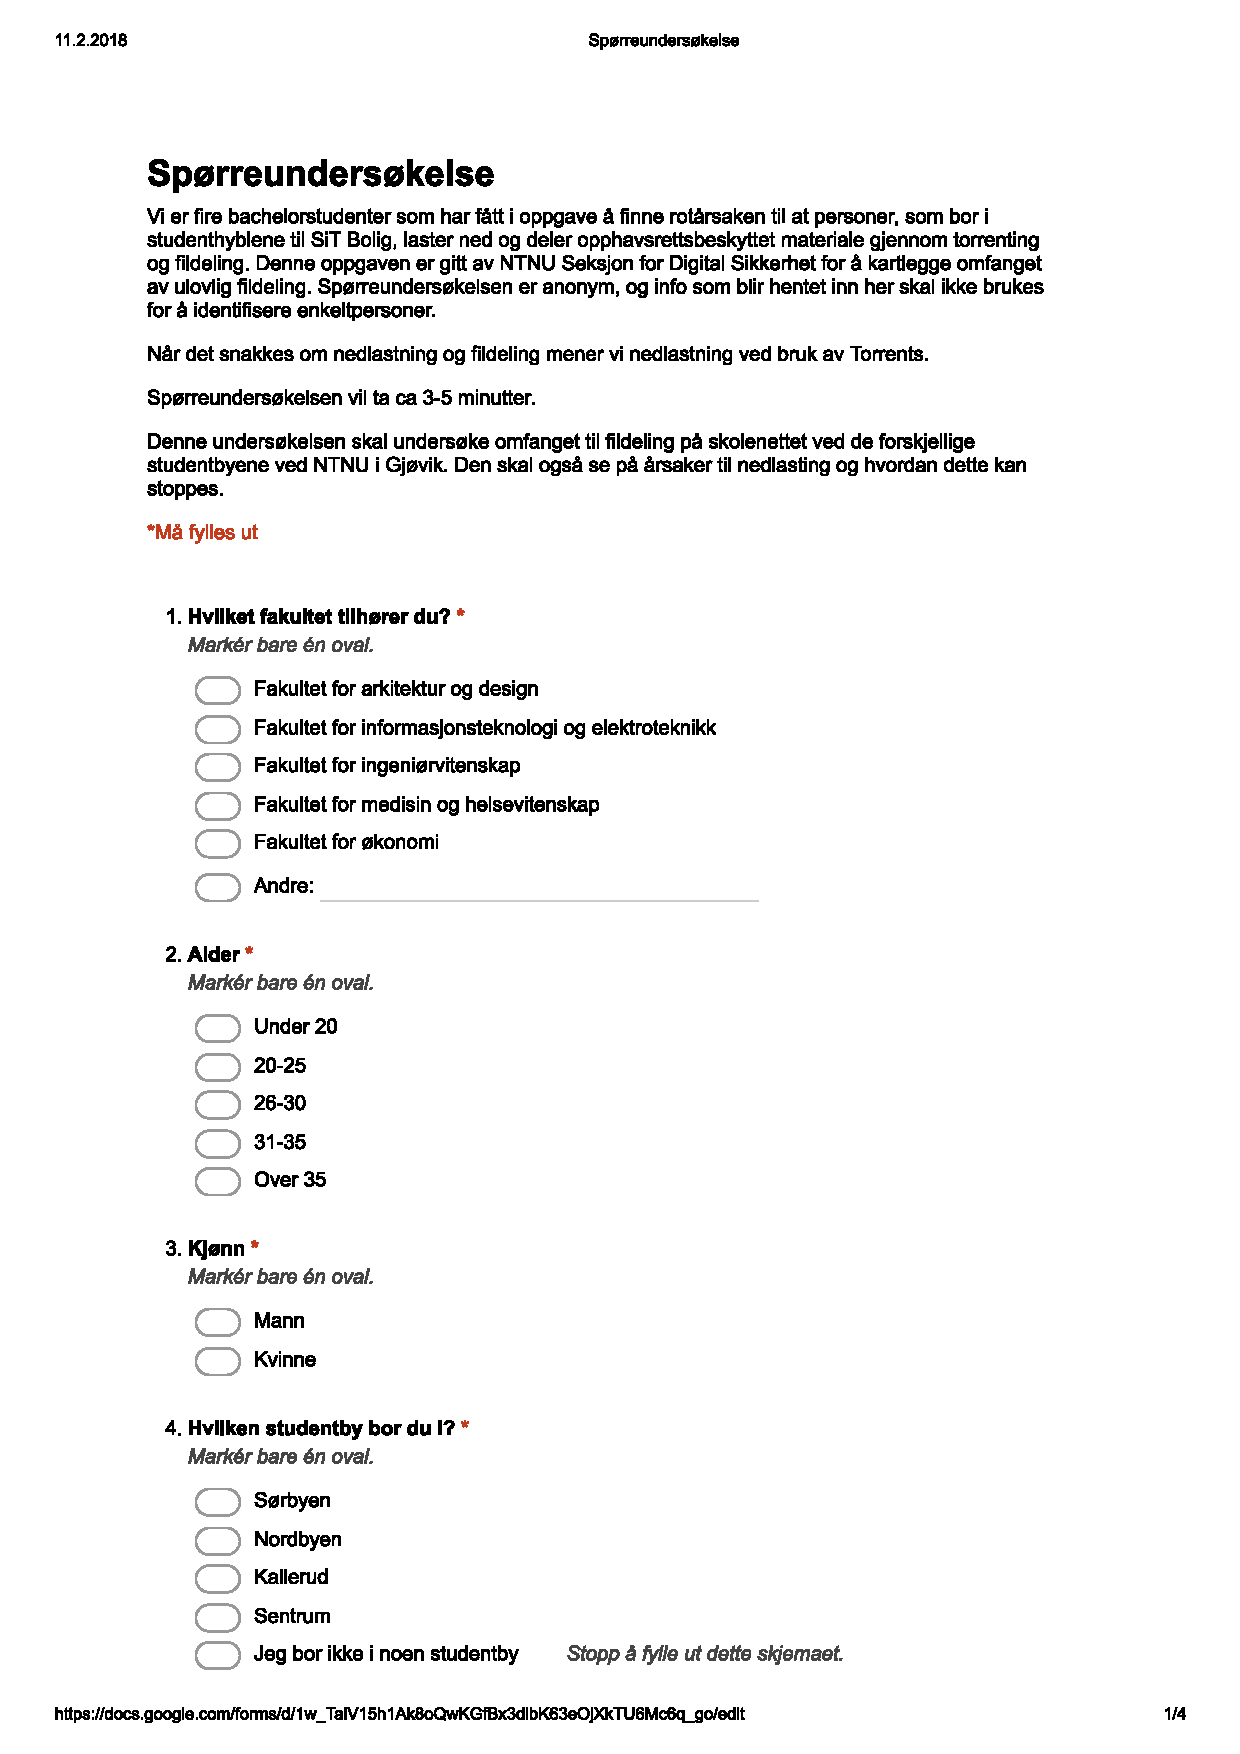
\includepdf[pages={1-4}]{bilder/case1_sporreundersokelse}

\chapter*{Vedlegg B: Plakat}
\label{plakat}
\begin{figure}[H]
    \centering
    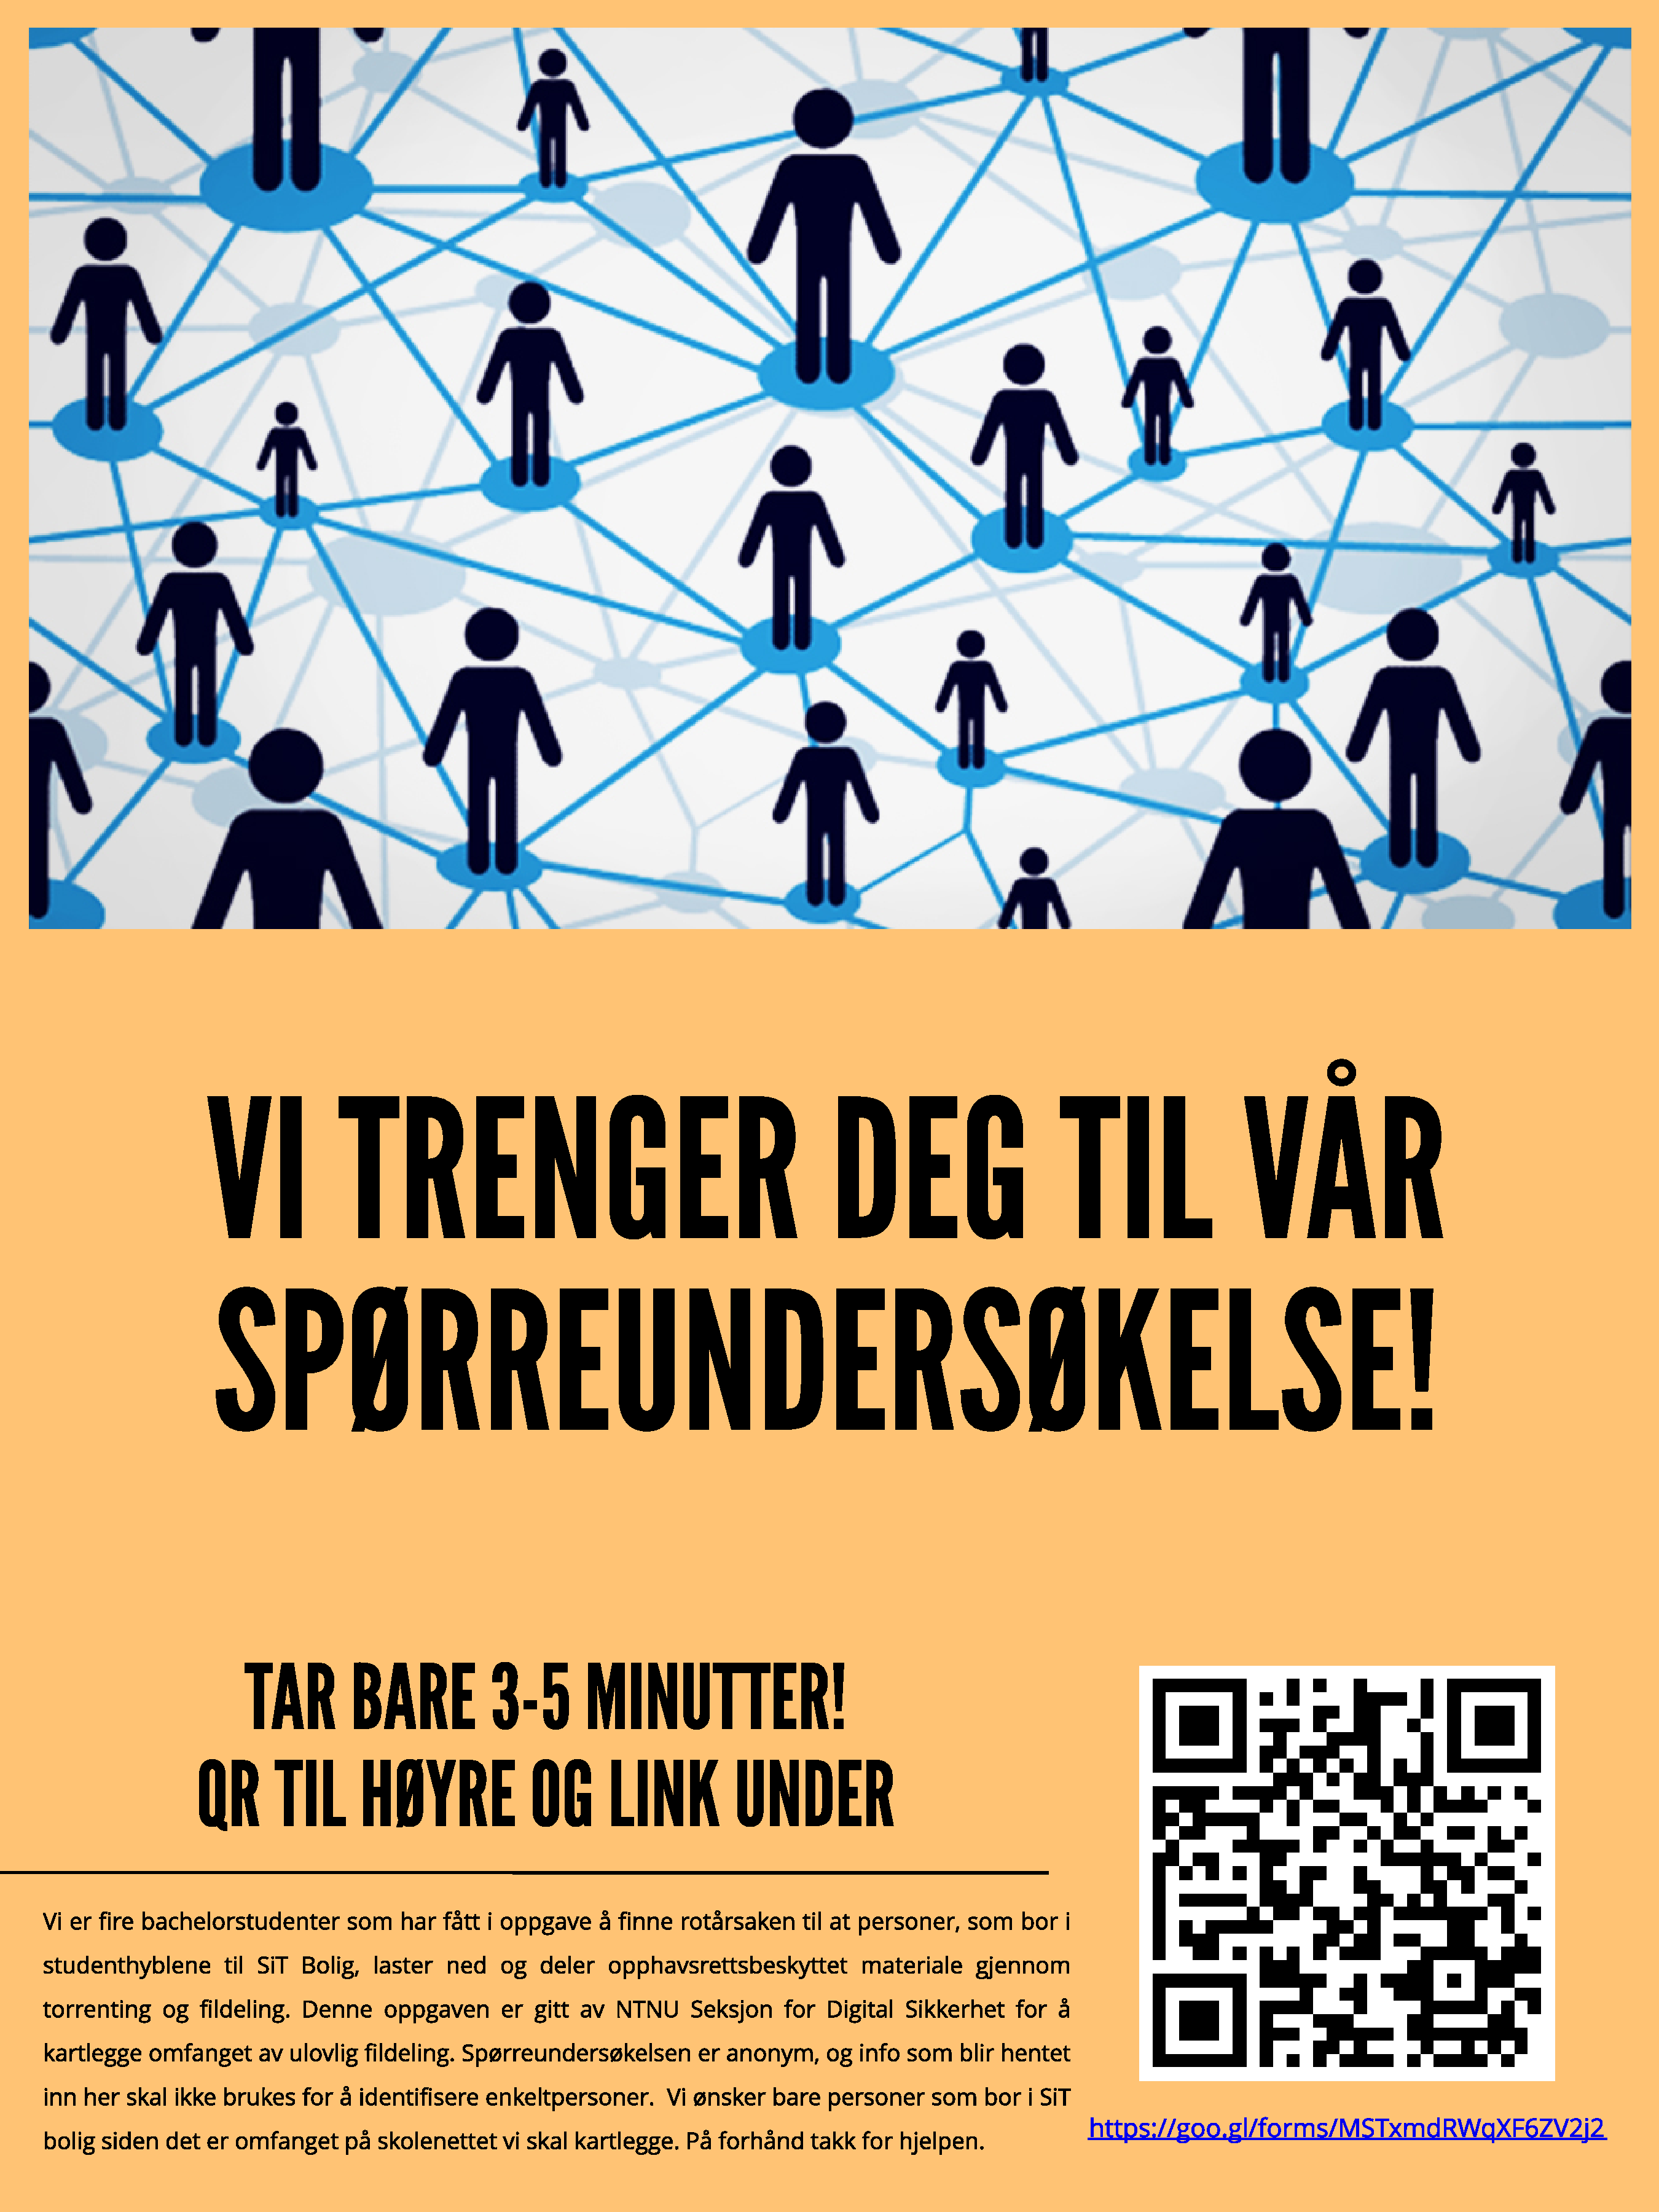
\includegraphics[scale=0.25]{case_1/bilder/plakat.pdf}
    \caption[Plakat]{Plakat som ble brukt i forbindelse med promotering av spørreundersøkelsen}
    \label{fig:plakat}
\end{figure}

\chapter*{Vedlegg C: Frekvenstabeller}
\label{frekvens}

% Table generated by Excel2LaTeX from sheet 'Ark1'
\begin{table}[htbp]
  \centering
    \begin{tabular}{|l|r|r|r|l|}
    \hline
    \multicolumn{5}{|p{30em}|}{\textcolor[rgb]{ .6,  .2,  0}{\textbf{\begin{center}Kjønn\end{center}}}} \\
    \hline
    \textcolor[rgb]{ .2,  .2,  .6}{} & \multicolumn{1}{p{5.355em}|}{\textcolor[rgb]{ .2,  .2,  .6}{Frequency}} & \multicolumn{1}{p{5.355em}|}{\textcolor[rgb]{ .2,  .2,  .6}{Percent}} & \multicolumn{1}{p{5.355em}|}{\textcolor[rgb]{ .2,  .2,  .6}{Valid Percent}} & \multicolumn{1}{p{5.355em}|}{\textcolor[rgb]{ .2,  .2,  .6}{Cumulative Percent}} \\
    \hline
    \textcolor[rgb]{ .2,  .2,  .6}{Kvinne} & \textcolor[rgb]{ .6,  .2,  0}{27} & \textcolor[rgb]{ .6,  .2,  0}{27.8} & \textcolor[rgb]{ .6,  .2,  0}{27.8} & \multicolumn{1}{r|}{\textcolor[rgb]{ .6,  .2,  0}{27.8}} \\
    \hline
    \textcolor[rgb]{ .2,  .2,  .6}{Mann}  & \textcolor[rgb]{ .6,  .2,  0}{70} & \textcolor[rgb]{ .6,  .2,  0}{72.2} & \textcolor[rgb]{ .6,  .2,  0}{72.2} & \multicolumn{1}{r|}{\textcolor[rgb]{ .6,  .2,  0}{100.0}} \\
    \hline
    \textcolor[rgb]{ .2,  .2,  .6}{Total} & \textcolor[rgb]{ .6,  .2,  0}{97} & \textcolor[rgb]{ .6,  .2,  0}{100.0} & \textcolor[rgb]{ .6,  .2,  0}{100.0} & \textcolor[rgb]{ .6,  .2,  0}{} \\
    \hline
    \end{tabular}%
  \caption{Frekvenstabell av kjønn}
  \label{tab:kjonn}%
\end{table}%

\begin{table}[htbp]
  \centering
    \begin{tabular}{|l|r|r|r|l|}
    \hline
    \multicolumn{5}{|p{30em}|}{\textcolor[rgb]{ .6,  .2,  0}{\textbf{\begin{center}Alder\end{center}}}} \\
    \hline
    \textcolor[rgb]{ .2,  .2,  .6}{} & \multicolumn{1}{p{5.355em}|}{\textcolor[rgb]{ .2,  .2,  .6}{Frequency}} & \multicolumn{1}{p{5.355em}|}{\textcolor[rgb]{ .2,  .2,  .6}{Percent}} & \multicolumn{1}{p{5.355em}|}{\textcolor[rgb]{ .2,  .2,  .6}{Valid Percent}} & \multicolumn{1}{p{5.355em}|}{\textcolor[rgb]{ .2,  .2,  .6}{Cumulative Percent}} \\
    \hline
    \textcolor[rgb]{ .2,  .2,  .6}{Under 20} & \textcolor[rgb]{ .6,  .2,  0}{9} & \textcolor[rgb]{ .6,  .2,  0}{9.3} & \textcolor[rgb]{ .6,  .2,  0}{9.3} & \multicolumn{1}{r|}{\textcolor[rgb]{ .6,  .2,  0}{9.3}} \\
    \hline
    \textcolor[rgb]{ .2,  .2,  .6}{20-25}  & \textcolor[rgb]{ .6,  .2,  0}{72} & \textcolor[rgb]{ .6,  .2,  0}{74.2} & \textcolor[rgb]{ .6,  .2,  0}{74.2} & \multicolumn{1}{r|}{\textcolor[rgb]{ .6,  .2,  0}{83.5}} \\
    \hline
    \textcolor[rgb]{ .2,  .2,  .6}{26-30} & \textcolor[rgb]{ .6,  .2,  0}{11} & \textcolor[rgb]{ .6,  .2,  0}{11.3} & \textcolor[rgb]{ .6,  .2,  0}{11.3} & \multicolumn{1}{r|}{\textcolor[rgb]{ .6,  .2,  0}{94.9}} \\
    \hline
    \textcolor[rgb]{ .2,  .2,  .6}{31-35} & \textcolor[rgb]{ .6,  .2,  0}{4} & \textcolor[rgb]{ .6,  .2,  0}{4.1} & \textcolor[rgb]{ .6,  .2,  0}{4.1} & \multicolumn{1}{r|}{\textcolor[rgb]{ .6,  .2,  0}{99.0}} \\
    \hline
    \textcolor[rgb]{ .2,  .2,  .6}{Over 35} & \textcolor[rgb]{ .6,  .2,  0}{1} & \textcolor[rgb]{ .6,  .2,  0}{1.0} & \textcolor[rgb]{ .6,  .2,  0}{1.0} & \multicolumn{1}{r|}{\textcolor[rgb]{ .6,  .2,  0}{100.0}} \\
    \hline
    \textcolor[rgb]{ .2,  .2,  .6}{Total} & \textcolor[rgb]{ .6,  .2,  0}{97} & \textcolor[rgb]{ .6,  .2,  0}{100.0} & \textcolor[rgb]{ .6,  .2,  0}{100.0} & \multicolumn{1}{r|}{\textcolor[rgb]{ .6,  .2,  0}{}} \\
    \hline
    \end{tabular}%
  \caption{Frekvenstabell av alder}
  \label{tab:alder}%
\end{table}%

\begin{table}[htbp]
  \centering
    \begin{tabular}{|l|r|r|r|l|}
    \hline
    \multicolumn{5}{|p{30em}|}{\textcolor[rgb]{ .6,  .2,  0}{\textbf{\begin{center}Studentby\end{center}}}} \\
    \hline
    \textcolor[rgb]{ .2,  .2,  .6}{} & \multicolumn{1}{p{5.355em}|}{\textcolor[rgb]{ .2,  .2,  .6}{Frequency}} & \multicolumn{1}{p{5.355em}|}{\textcolor[rgb]{ .2,  .2,  .6}{Percent}} & \multicolumn{1}{p{5.355em}|}{\textcolor[rgb]{ .2,  .2,  .6}{Valid Percent}} & \multicolumn{1}{p{5.355em}|}{\textcolor[rgb]{ .2,  .2,  .6}{Cumulative Percent}} \\
    \hline
    \textcolor[rgb]{ .2,  .2,  .6}{Kallerud} & \textcolor[rgb]{ .6,  .2,  0}{49} & \textcolor[rgb]{ .6,  .2,  0}{50.5} & \textcolor[rgb]{ .6,  .2,  0}{50.5} & \multicolumn{1}{r|}{\textcolor[rgb]{ .6,  .2,  0}{50.5}} \\
    \hline
    \textcolor[rgb]{ .2,  .2,  .6}{Nordbyen}  & \textcolor[rgb]{ .6,  .2,  0}{13} & \textcolor[rgb]{ .6,  .2,  0}{13.4} & \textcolor[rgb]{ .6,  .2,  0}{13.4} & \multicolumn{1}{r|}{\textcolor[rgb]{ .6,  .2,  0}{63.9}} \\
    \hline
    \textcolor[rgb]{ .2,  .2,  .6}{Sentrum} & \textcolor[rgb]{ .6,  .2,  0}{11} & \textcolor[rgb]{ .6,  .2,  0}{11.3} & \textcolor[rgb]{ .6,  .2,  0}{11.3} & \multicolumn{1}{r|}{\textcolor[rgb]{ .6,  .2,  0}{75.3}} \\
    \hline
    \textcolor[rgb]{ .2,  .2,  .6}{Sørbyen} & \textcolor[rgb]{ .6,  .2,  0}{24} & \textcolor[rgb]{ .6,  .2,  0}{24.7} & \textcolor[rgb]{ .6,  .2,  0}{24.7} & \multicolumn{1}{r|}{\textcolor[rgb]{ .6,  .2,  0}{100.0}} \\
    \hline
    \textcolor[rgb]{ .2,  .2,  .6}{Total} & \textcolor[rgb]{ .6,  .2,  0}{97} & \textcolor[rgb]{ .6,  .2,  0}{100.0} & \textcolor[rgb]{ .6,  .2,  0}{100.0} & \multicolumn{1}{r|}{\textcolor[rgb]{ .6,  .2,  0}{}} \\
    \hline
    \end{tabular}%
  \caption{Frekvenstabell av studentby}
  \label{tab:studentby}%
\end{table}%

\begin{table}[htbp]
  \centering
    \begin{tabular}{|p{5.355em}|r|r|r|l|}
    \hline
    \multicolumn{5}{|p{30em}|}{\textcolor[rgb]{ .6,  .2,  0}{\textbf{\begin{center}Fakultet\end{center}}}} \\
    \hline
    \multicolumn{1}{|r|}{\textcolor[rgb]{ .2,  .2,  .6}{}} & \multicolumn{1}{p{5.355em}|}{\textcolor[rgb]{ .2,  .2,  .6}{Frequency}} & \multicolumn{1}{p{5.355em}|}{\textcolor[rgb]{ .2,  .2,  .6}{Percent}} & \multicolumn{1}{p{5.355em}|}{\textcolor[rgb]{ .2,  .2,  .6}{Valid Percent}} & \multicolumn{1}{p{5.355em}|}{\textcolor[rgb]{ .2,  .2,  .6}{Cumulative Percent}} \\
    \hline
    \textcolor[rgb]{ .2,  .2,  .6}{Fakultet for arkitektur og design} & \textcolor[rgb]{ .6,  .2,  0}{15} & \textcolor[rgb]{ .6,  .2,  0}{15.5} & \textcolor[rgb]{ .6,  .2,  0}{15.5} & \multicolumn{1}{r|}{\textcolor[rgb]{ .6,  .2,  0}{15.5}} \\
    \hline
    \textcolor[rgb]{ .2,  .2,  .6}{Fakultet for informasjonsteknologi og elektroteknikk} & \textcolor[rgb]{ .6,  .2,  0}{52} & \textcolor[rgb]{ .6,  .2,  0}{53.6} & \textcolor[rgb]{ .6,  .2,  0}{53.6} & \multicolumn{1}{r|}{\textcolor[rgb]{ .6,  .2,  0}{69.1}} \\
    \hline
    \textcolor[rgb]{ .2,  .2,  .6}{Fakultet for ingeniørvitenskap} & \textcolor[rgb]{ .6,  .2,  0}{13} & \textcolor[rgb]{ .6,  .2,  0}{13.4} & \textcolor[rgb]{ .6,  .2,  0}{13.4} & \multicolumn{1}{r|}{\textcolor[rgb]{ .6,  .2,  0}{82.5}} \\
    \hline
    \textcolor[rgb]{ .2,  .2,  .6}{Fakultet for medisin og helsevitenskap} & \textcolor[rgb]{ .6,  .2,  0}{11} & \textcolor[rgb]{ .6,  .2,  0}{11.3} & \textcolor[rgb]{ .6,  .2,  0}{11.3} & \multicolumn{1}{r|}{\textcolor[rgb]{ .6,  .2,  0}{93.8}} \\
    \hline
    \textcolor[rgb]{ .2,  .2,  .6}{Fakultet for økonomi} & \textcolor[rgb]{ .6,  .2,  0}{6} & \textcolor[rgb]{ .6,  .2,  0}{6.2} & \textcolor[rgb]{ .6,  .2,  0}{6.2} & \multicolumn{1}{r|}{\textcolor[rgb]{ .6,  .2,  0}{100.0}} \\   
    \hline
    \textcolor[rgb]{ .2,  .2,  .6}{Total} & \textcolor[rgb]{ .6,  .2,  0}{97} & \textcolor[rgb]{ .6,  .2,  0}{100.0} & \textcolor[rgb]{ .6,  .2,  0}{100.0} & \textcolor[rgb]{ .6,  .2,  0}{} \\
    \hline
    \end{tabular}%
  \caption{Frekvenstabell av fakultet}
  \label{tab:fakultet}%
\end{table}%

\chapter*{Vedlegg D: Diverse Histogrammer}
\label{vedlegg:histogrammer}

\begin{figure}[H]
    \centering
    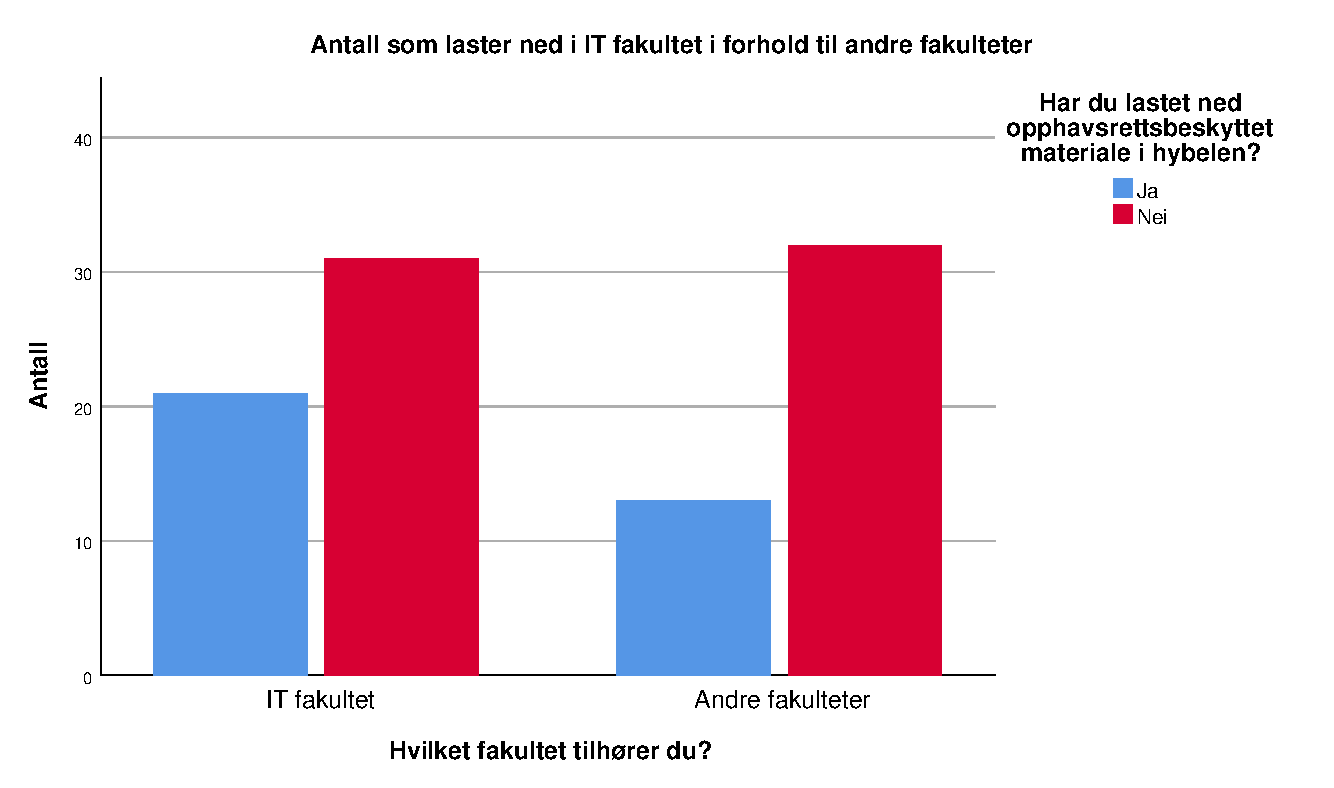
\includegraphics[scale=0.45]{case_1/bilder/IT_lasterned.pdf}
    \caption[IT-lasterned]{Forholdet mellom IT studier og andre når det kommer til nedlasting}
    \label{fig:IT-lasterned}
\end{figure}

\begin{figure}[H]
    \centering
    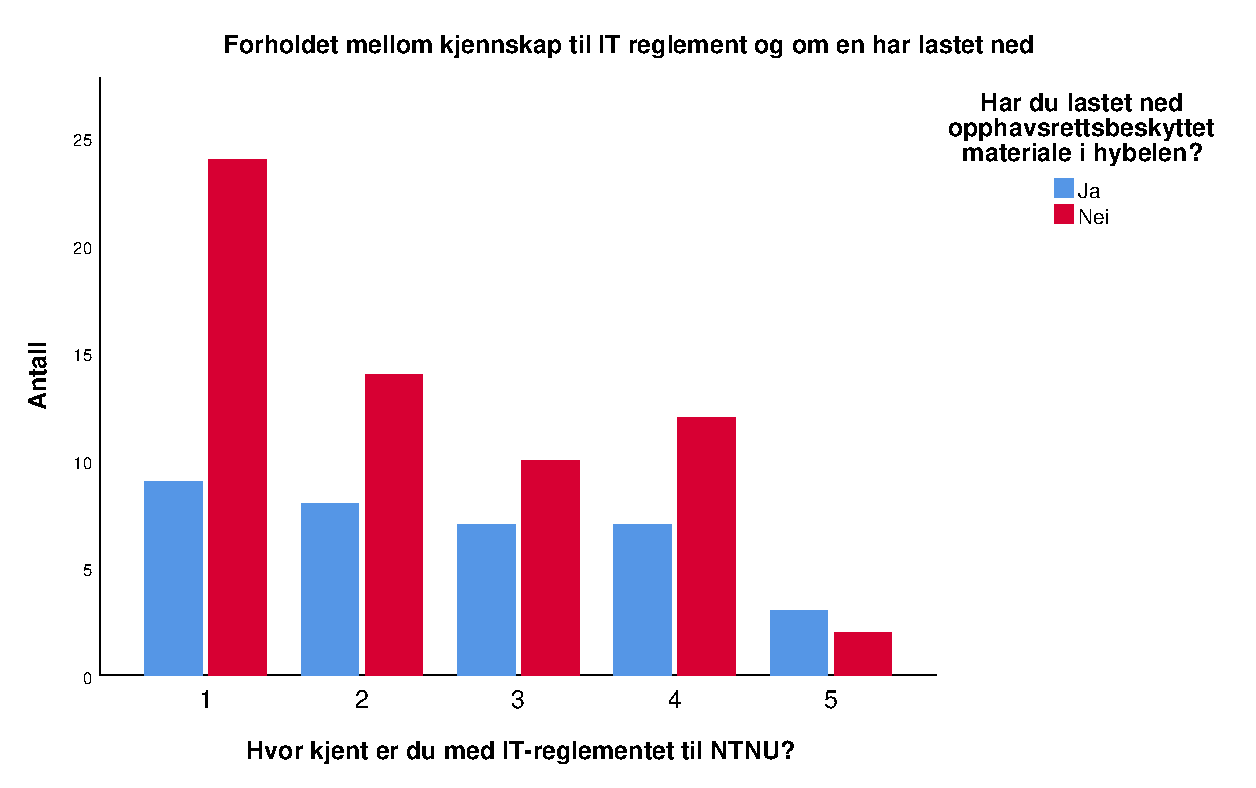
\includegraphics[scale=0.45]{case_1/bilder/reglement_lasterned.pdf}
    \caption[reglement-lasterned]{Forholdet mellom kjennskap til IT reglement og om en laster ned}
    \label{fig:reglement-lasterned}
\end{figure}

\begin{figure}[H]
    \centering
    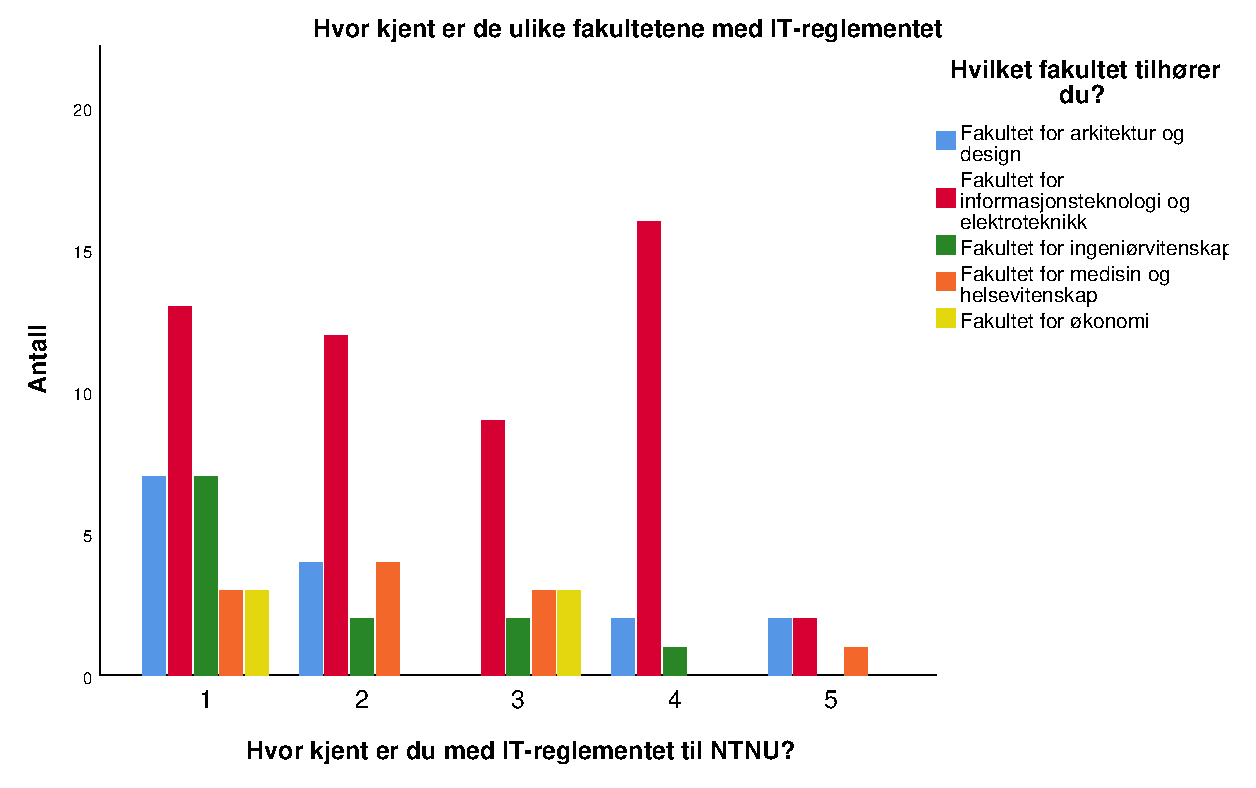
\includegraphics[scale=0.45]{case_1/bilder/reglement_fakultet.pdf}
    \caption[reglement-fakultet]{Hvor godt kjennskap de ulike fakultetene har med IT reglementet}
    \label{fig:reglement-fakultet}
\end{figure}

\begin{figure}[H]
    \centering
    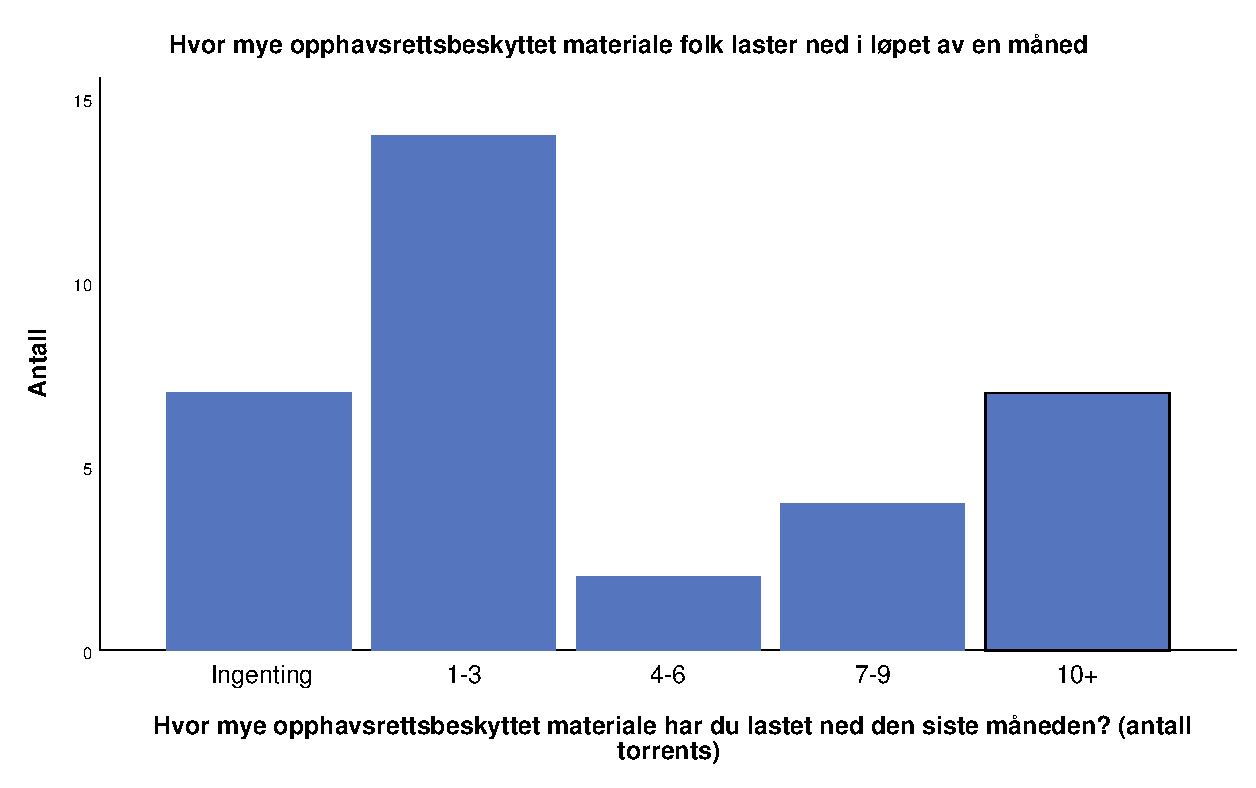
\includegraphics[scale=0.45]{case_1/bilder/antalltorrents.pdf}
    \caption[antalltorrents]{Hvor mange torrents folk laster ned i løpet av en måned}
    \label{fig:antalltorrents}
\end{figure}

\chapter*{Vedlegg E: SPSS analyser}
\label{vedlegg:ANOVA}

%-----------------------------------------------ONEWAY ANOVA - FAKULTET MOT PÅSTAND------------------------
%-----------------------------------------------DESCRIPTIVES-----------------------------------------------
\begin{figure}[H]
    \centering
    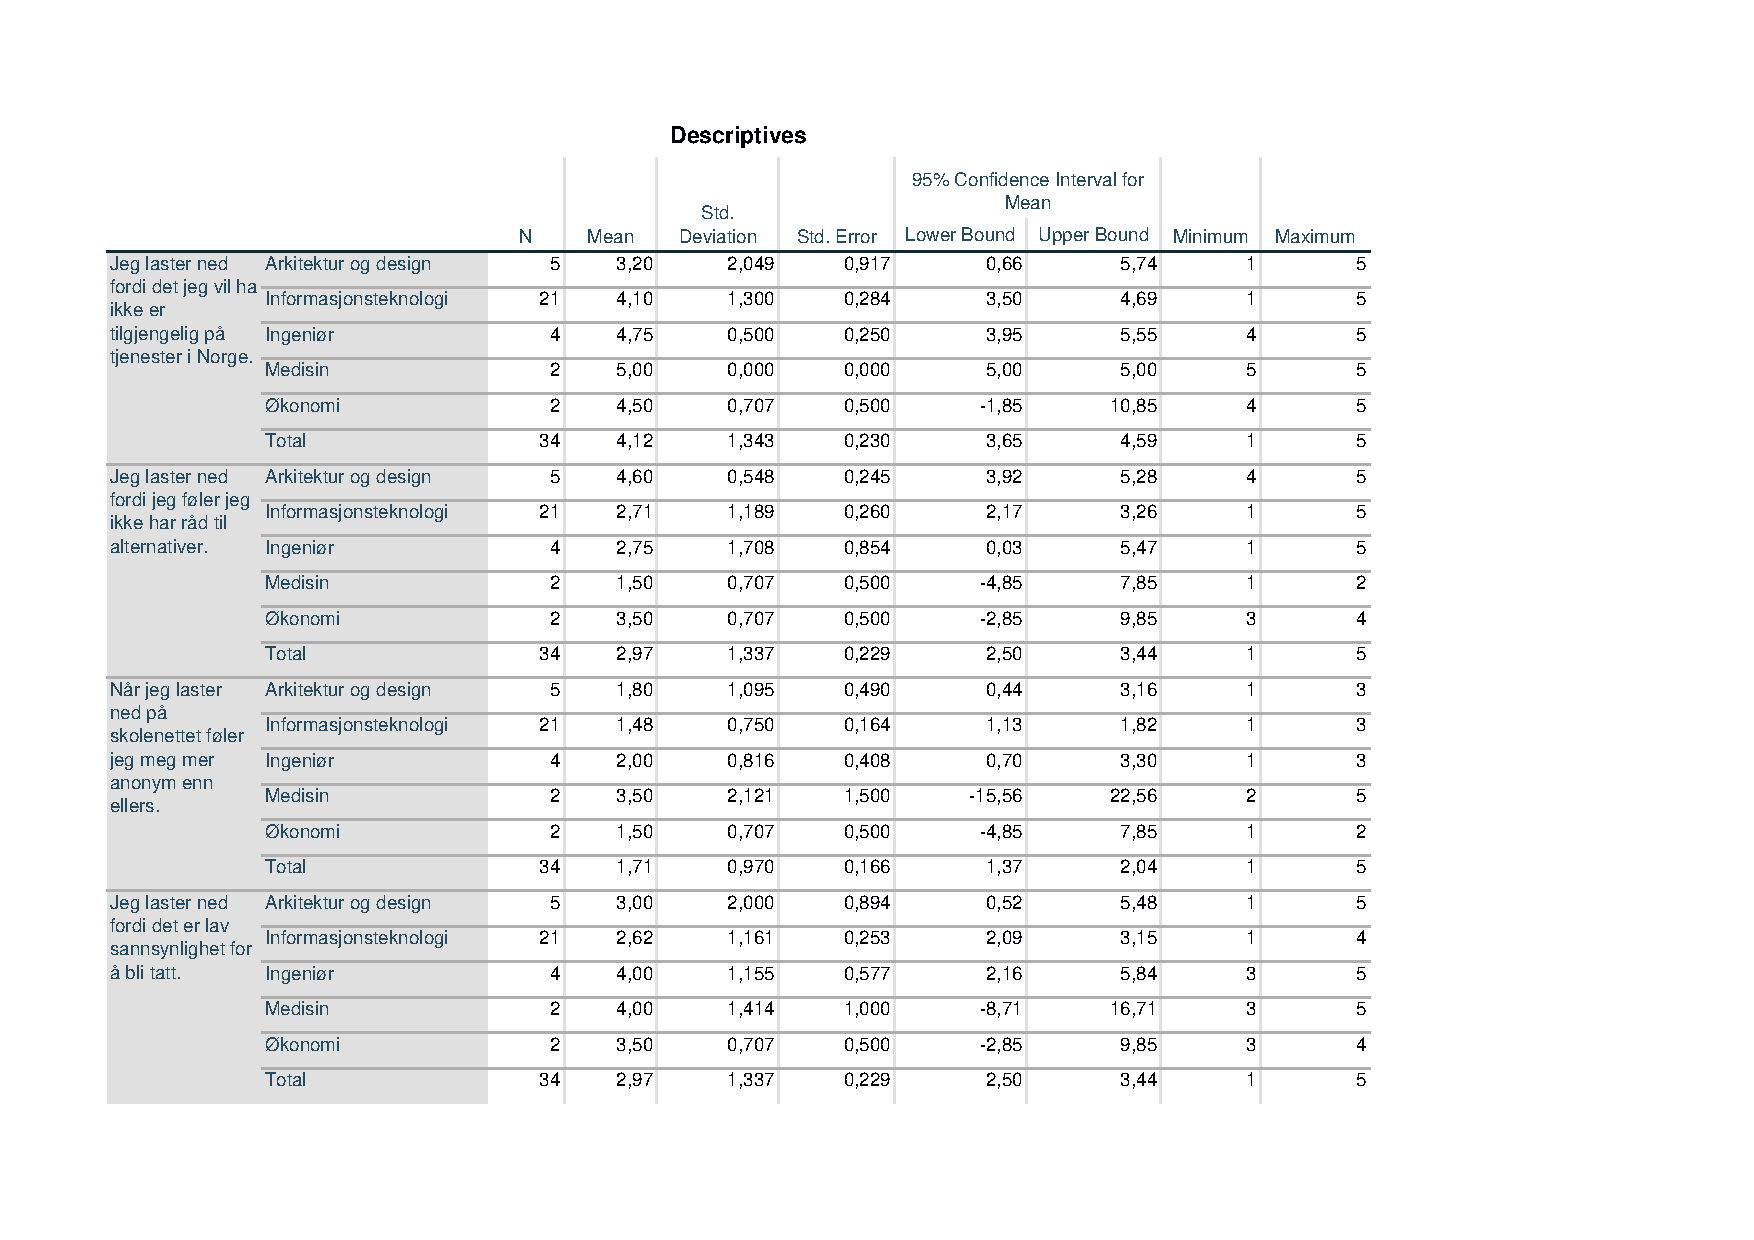
\includegraphics[scale=0.7]{case_1/bilder/DESCRIPTIVES_fakultet-pastand_LIGGENDE.pdf}
    \label{fig:DESCRIPTIVES_fakultet-påstand}
    \caption{Fakultet mot påstander}
\end{figure}


%-----------------------------------------------ANOVA-------------------------------------------------------
\begin{figure}[H]
    \centering
    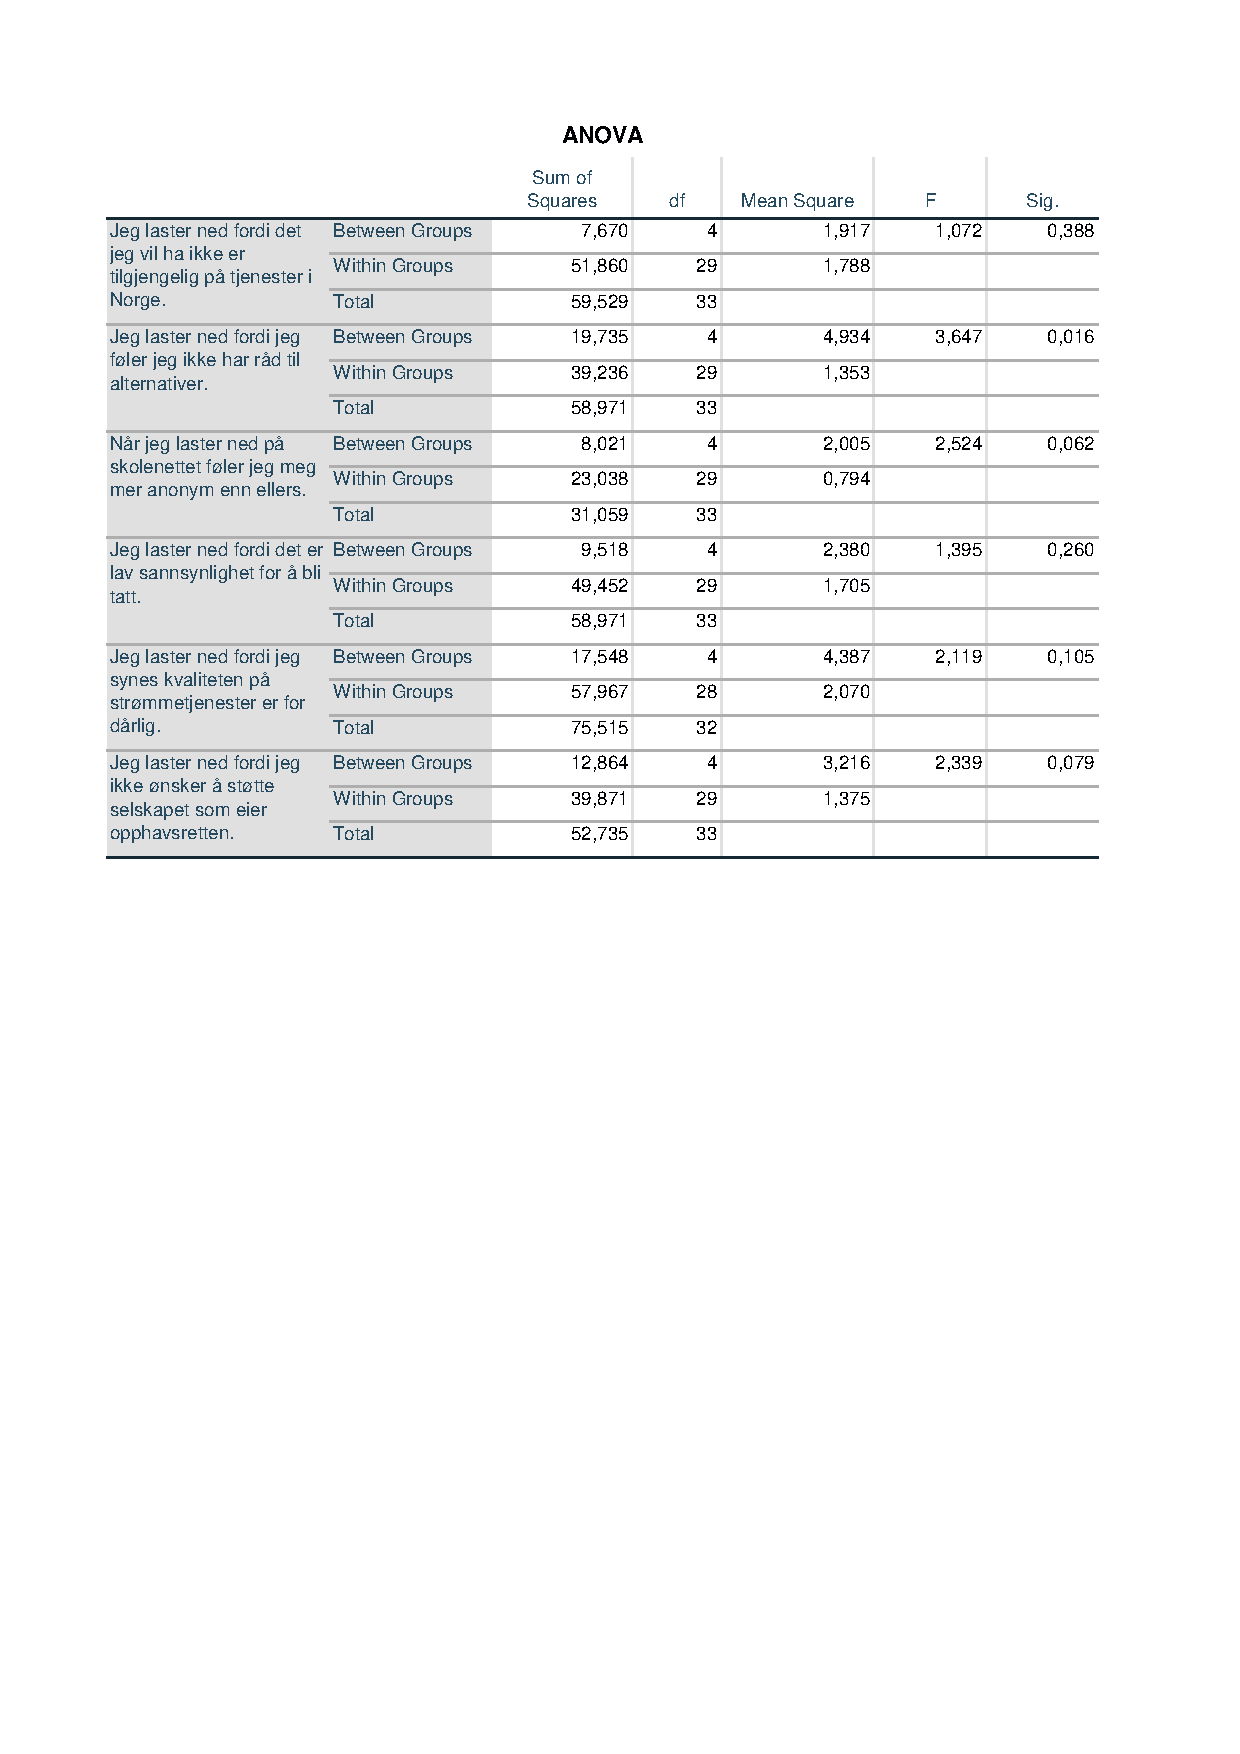
\includegraphics[scale=0.7]{case_1/bilder/ANOVA_fakultet-pastand.pdf}
    \label{fig:ANOVA_fakultet-påstand}
    \caption{Fakultet mot påstander - ANOVA}
\end{figure}


%-----------------------------------------------POST HOC ANALYSE--------------------------------------------
\begin{figure}[H]
    \centering
    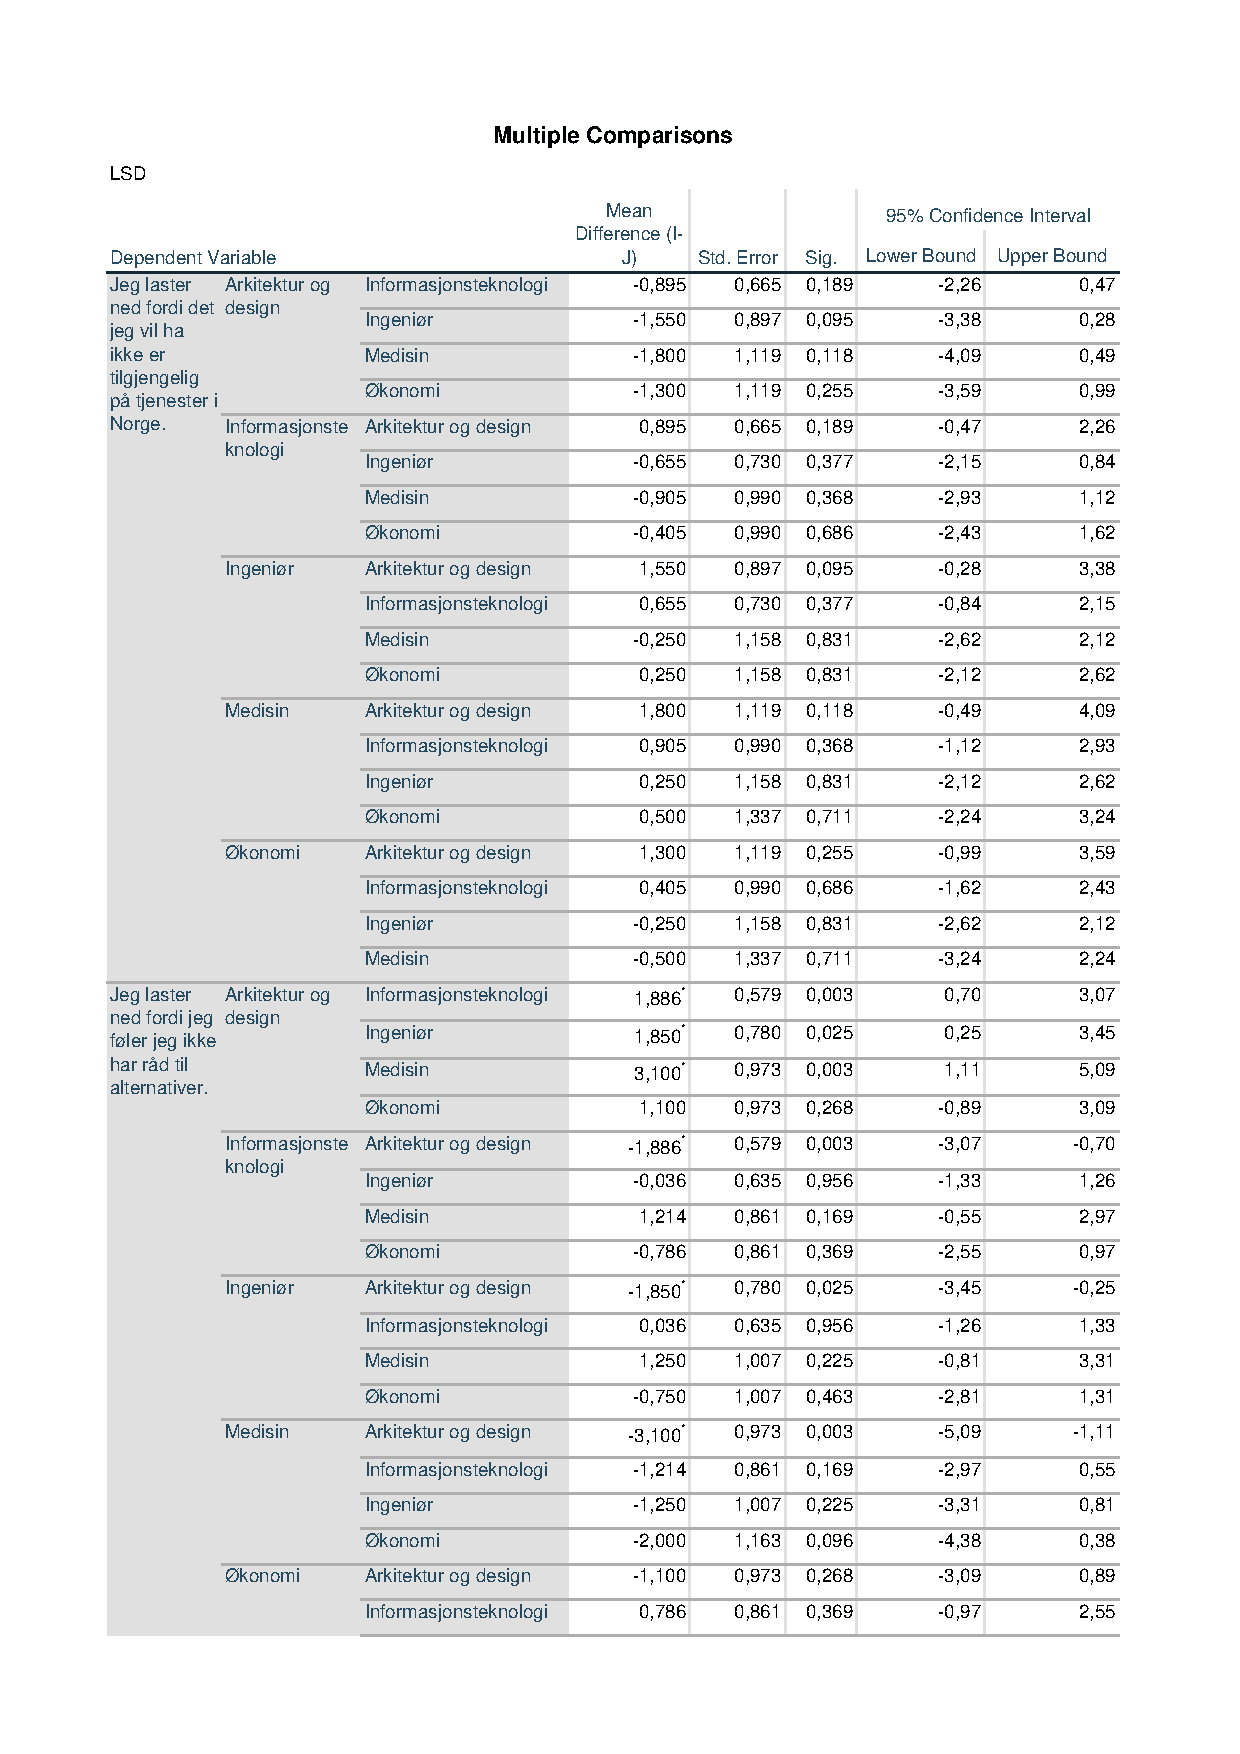
\includegraphics[scale=0.7]{case_1/bilder/Post_Hoc_test_fakultet-pastand.pdf}
    \label{fig:POST-HOC_fakultet-påstand}
    \caption{Fakultet mot påstander - POST HOC}
\end{figure}



%-----------------------------------------------ONEWAY ANOVA - IT/ANDRE MOT PÅSTAND------------------------
%-----------------------------------------------DESCRIPTIVES-----------------------------------------------
\begin{figure}[H]
    \centering
    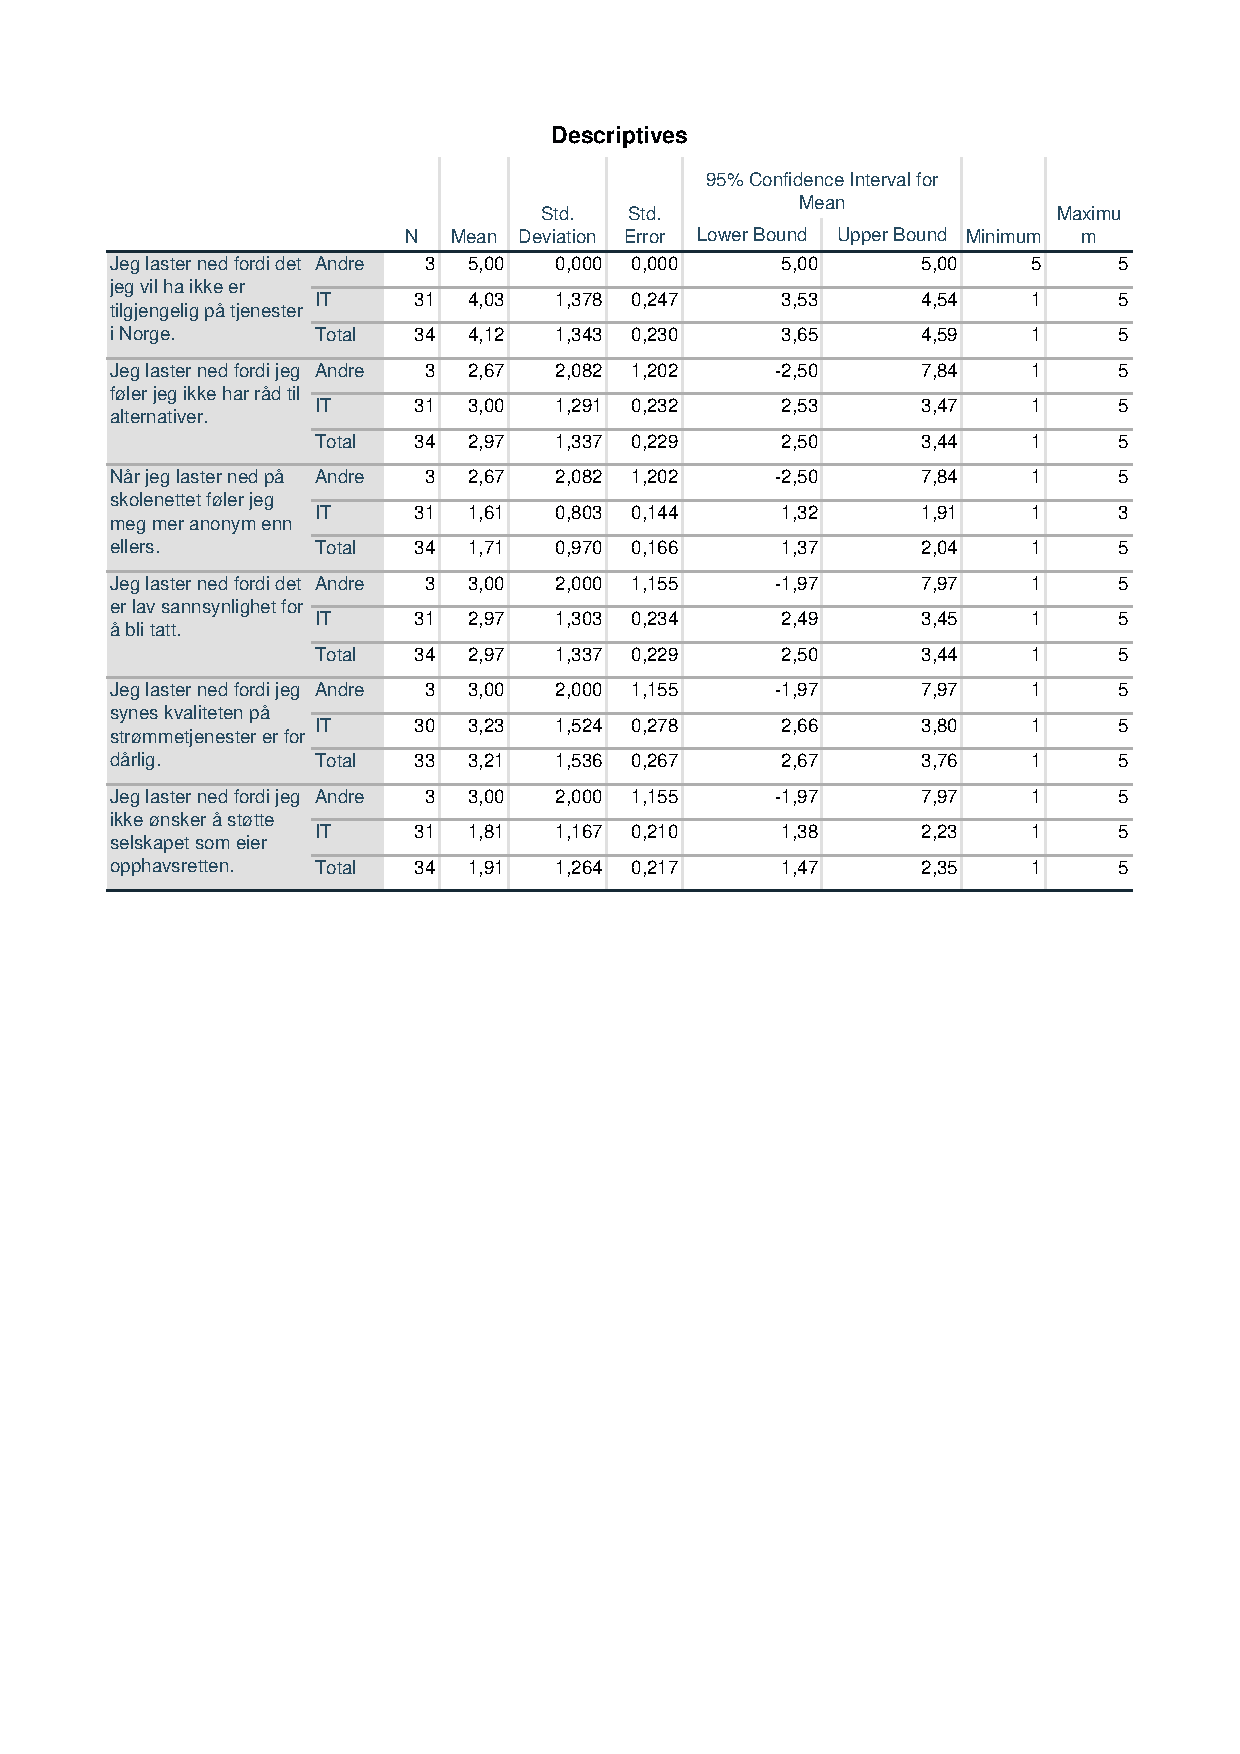
\includegraphics[scale=0.7]{case_1/bilder/DESCRIPTIVES_IT-ANDRE-pastand.pdf}
    \label{fig:DESCRIPTIVES_IT/ANDRE-påstand}
    \caption{Fakultet delt inn i IT og andre mot påstander - DESCRIPTIVES}
    
\end{figure}

%-----------------------------------------------ANOVA-------------------------------------------------------
\begin{figure}[H]
    \centering
    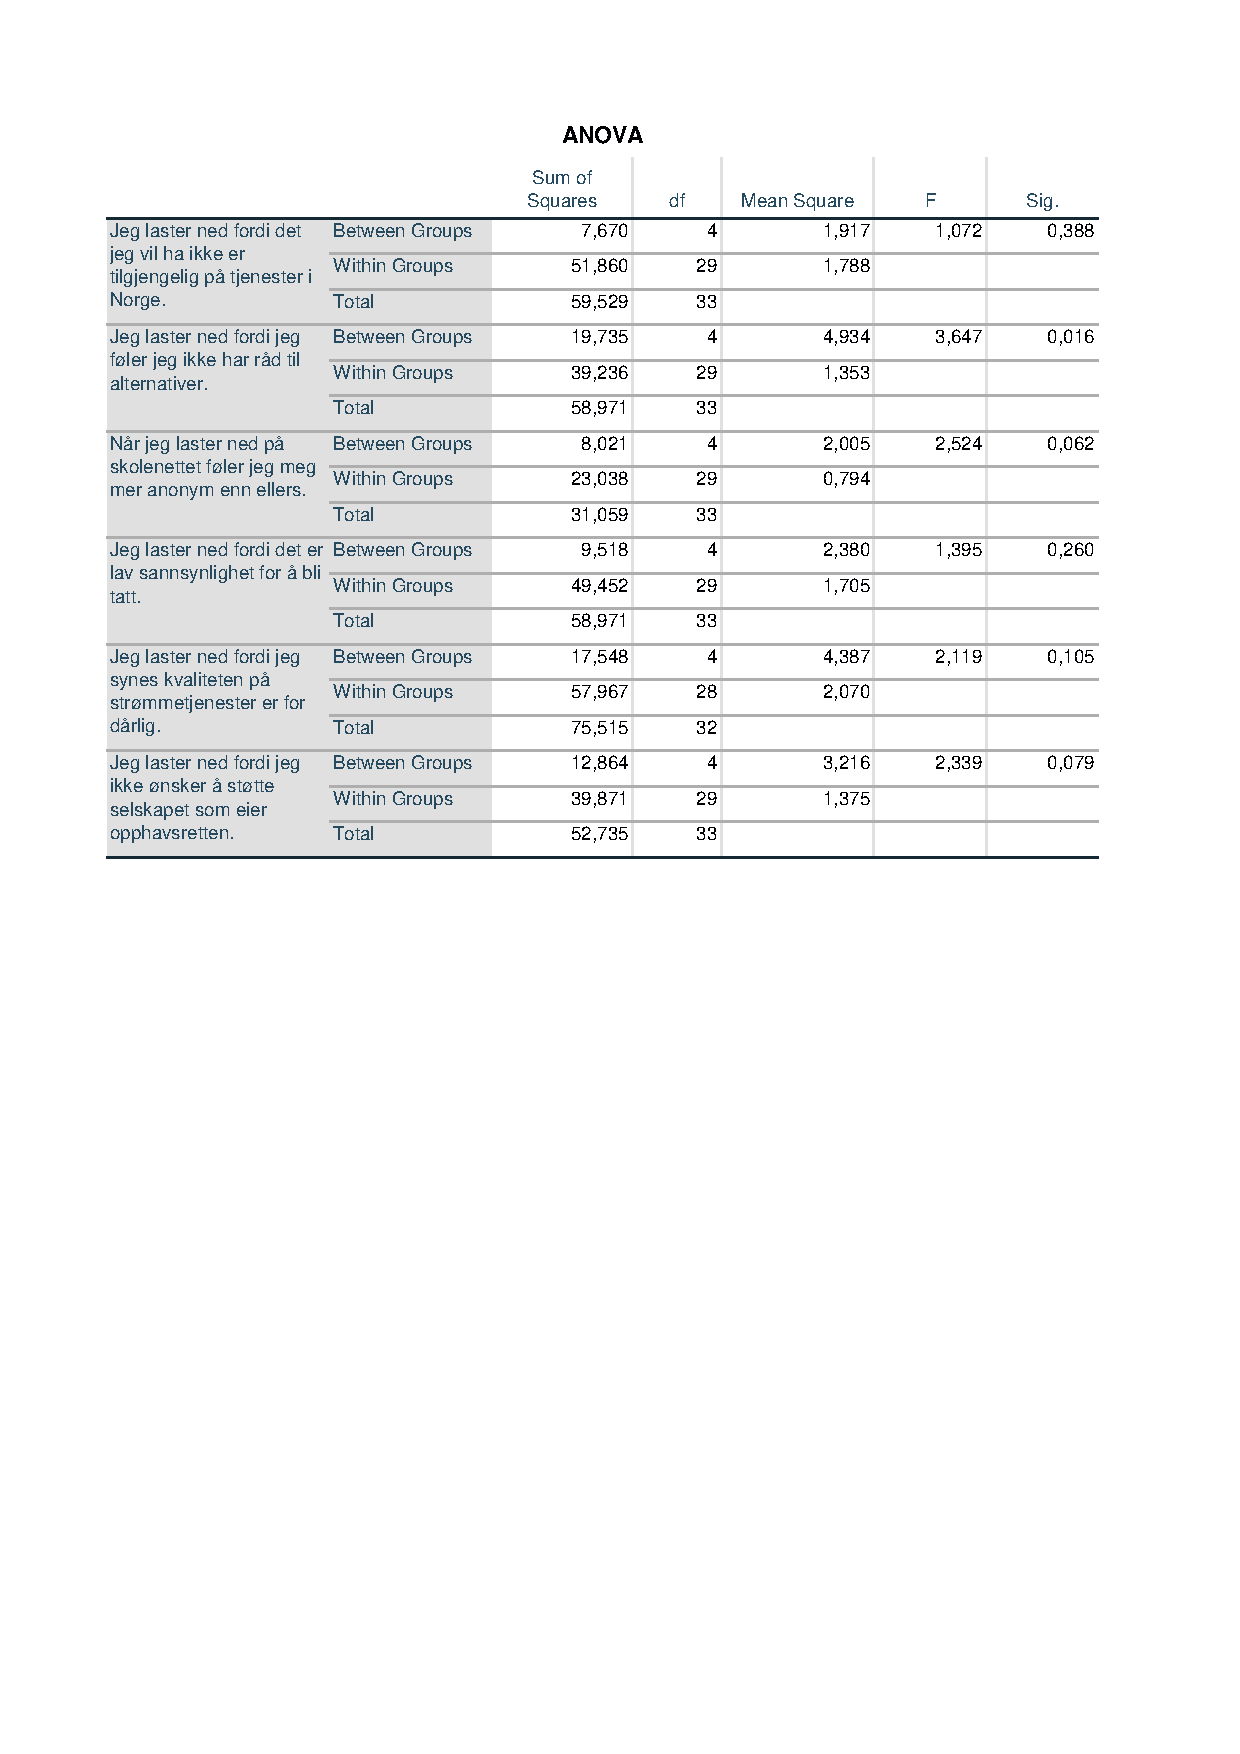
\includegraphics[scale=0.7]{case_1/bilder/ANOVA_fakultet-pastand.pdf}
    \label{fig:ANOVA_IT/ANDRE-påstand}
    \caption{Fakultet delt inn i IT og andre mot påstander - ANOVA}
\end{figure}




\end{document}